% ----------------------------------------------------------------------------------------------------------
% Packages
% ----------------------------------------------------------------------------------------------------------

\documentclass[12pt,a4paper,bibliography=totocnumbered,listof=totocnumbered]{scrartcl}
\usepackage[english]{babel}
\usepackage[utf8]{inputenc}
\usepackage{amsmath}
\usepackage{amsfonts}
\usepackage{amssymb}
\usepackage{graphicx}
\usepackage{fancyhdr}
\usepackage{tabularx}
\usepackage{geometry}
\usepackage{setspace}
\usepackage[right]{eurosym}
\usepackage[printonlyused]{acronym}
\usepackage{subfig}
\usepackage{floatflt}
\usepackage[usenames,dvipsnames]{color}
\usepackage{colortbl}
\usepackage{paralist}
\usepackage{array}
\usepackage{titlesec}
%\usepackage{dsfont}
\usepackage{parskip}
\usepackage[right]{eurosym}
\usepackage[subfigure,titles]{tocloft}
\usepackage[pdfpagelabels=true]{hyperref}
\usepackage{mathdots}
\usepackage{listings}
\usepackage{lipsum}
\usepackage{booktabs}
\usepackage{fix-cm}
\usepackage{rotating}
\usepackage{pdflscape}
\usepackage{bbold}
\usepackage[labelfont=bf]{caption}
\captionsetup{labelfont=bf}
\usepackage{tikz}
\usepackage{breakcites}
\usepackage{float}
\usepackage{tcolorbox}
 \usepackage[flushleft]{threeparttable}
% ----------------------------------------------------------------------------------------------------------
% Packages
% ----------------------------------------------------------------------------------------------------------


\lstset{basicstyle=\footnotesize, captionpos=t, breaklines=true, showstringspaces=false, tabsize=2, frame=lines, numbers=left, numberstyle=\tiny, xleftmargin=2em, framexleftmargin=2em}
\makeatletter
\def\l@lstlisting#1#2{\@dottedtocline{1}{0em}{1em}{\hspace{1,5em} Lst. #1}{#2}}
\makeatother



\geometry{a4paper, top=27mm, left=27mm, right=27mm, bottom=35mm, headsep=10mm, footskip=12mm}

% ----------------------------------------------------------------------------------------------------------
% Packages
% ----------------------------------------------------------------------------------------------------------


\hypersetup{unicode=false, pdftoolbar=true, pdfmenubar=true, pdffitwindow=false, pdfstartview={FitH},
	pdftitle={Master Thesis},
	pdfauthor={Felix Gutmann},
	pdfsubject={Bachelor Thesis},
	pdfcreator={\LaTeX\ with package \flqq hyperref\frqq},
	pdfproducer={pdfTeX \the\pdftexversion.\pdftexrevision},
	pdfkeywords={Bachelor Thesis},
	pdfnewwindow=true,
	colorlinks=true,linkcolor=black,citecolor=black,filecolor=magenta,urlcolor=black}
\pdfinfo{/CreationDate (D:20110620133321)}
\DeclareMathOperator*{\argmin}{arg\,min}



\begin{document}

\titlespacing\section{0pt}{12pt plus 4pt minus 2pt}{0pt plus 2pt minus 2pt}
\titlespacing\subsection{0pt}{30pt plus 4pt minus 2pt}{0pt plus 2pt minus 2pt}
\titlespacing\subsubsection{0pt}{12pt plus 4pt minus 2pt}{0pt plus 2pt minus 2pt}
% Headers and footers

\renewcommand{\sectionmark}[1]{\markright{#1}}
\renewcommand{\leftmark}{\rightmark}
\pagestyle{fancy}
\lhead{}
\chead{}
\rhead{\thesection\space\contentsname}
%\lfoot{Complex Economic Systems - An analytical approach to Input-Output tables\newline}
\cfoot{}
\rfoot{\ \linebreak \thepage}
\renewcommand{\headrulewidth}{0.4pt}
\renewcommand{\footrulewidth}{0.4pt}

% ----------------------------------------------------------------------------------------------------------
%Prefix
% ----------------------------------------------------------------------------------------------------------

\renewcommand{\thesection}{\Roman{section}}
\renewcommand{\theHsection}{\Roman{section}}
\pagenumbering{Roman}

% ----------------------------------------------------------------------------------------------------------
% Title
% ----------------------------------------------------------------------------------------------------------

\thispagestyle{empty}
\begin{center}
	
\includegraphics[width=\textwidth]{Pictures/logo01.jpg}\\
	\vspace*{2cm}
	\vspace*{2cm}
	\Huge
	\textbf{Master Thesis}\\
	\vspace*{0.5cm}
	\large
	\textbf{Topic:}\\
	\vspace*{1cm}
	\textbf{Unsupervised learning in decision making}\\
	\vspace*{2cm}
\end{center}	

$\vspace{6cm}$
\begin{tabbing}
\hspace*{1cm}\=\hspace*{3.2cm}\=\hspace*{3cm}\=\hspace*{2.7cm}\= \kill
\onehalfspacing
\textbf{Author:} \>\> Domagoj Fizulic\\
\textbf{} \>\> Felix Gutmann\\
\textbf{Student number:} 	\>\> 125604\\
\textbf{} 	\>\> 125584\\
\textbf{Program:} \>\> M.S. Data Science\\
\textbf{E-Mail:} \>\> domagoj.fizulic@barcelonagse.eu\\
\textbf{} \>\> felix.gutmann@barcelonagse.eu
\end{tabbing}
\vspace{1cm}


\pagebreak
% ----------------------------------------------------------------------------------------------------------
% Abstract
% ----------------------------------------------------------------------------------------------------------


\onehalfspacing




\pagebreak

% ----------------------------------------------------------------------------------------------------------
% Index
% ----------------------------------------------------------------------------------------------------------


\renewcommand{\cfttabpresnum}{Tab. }
\renewcommand{\cftfigpresnum}{Fig. }
\settowidth{\cfttabnumwidth}{Fig. 10\quad}
\settowidth{\cftfignumwidth}{Fig. 10\quad}

\titlespacing{\section}{0pt}{12pt plus 4pt minus 2pt}{2pt plus 2pt minus 2pt}
\singlespacing
\rhead{Table of contents}
\renewcommand{\contentsname}{I Table of Contents}
\phantomsection
\addcontentsline{toc}{section}{\texorpdfstring{I \hspace{0.35em}Table of Contents}{Table of Contents}}
\addtocounter{section}{1}


% ----------------------------------------------------------------------------------------------------------
% Table of contents
% ----------------------------------------------------------------------------------------------------------

\setcounter{page}{1}

\rhead{Table of Contents}

	\tableofcontents


\pagebreak
% ----------------------------------------------------------------------------------------------------------
% List of figures
% ----------------------------------------------------------------------------------------------------------

\rhead{List of Figures}

	\listoffigures
	
	
\pagebreak
% ----------------------------------------------------------------------------------------------------------
% List of tables
% ----------------------------------------------------------------------------------------------------------

\rhead{List of Tables}

	\listoftables
	

\pagebreak
%----------------------------------------------------------------------------------------------------------
% List of Listings
% ----------------------------------------------------------------------------------------------------------

\rhead{List of Listings}
\renewcommand{\lstlistlistingname}{List of Listings}
{\labelsep2cm\lstlistoflistings}
\pagebreak

%----------------------------------------------------------------------------------------------------------
% List of Symbols
% ---------------------------------------------------------------------------------------------------------

\renewcommand{\arraystretch}{1.5}	
\section{List of mathematical symbols}
\rhead{List of mathematical Symbols}

\begin{tabular}{p{6cm}p{9cm}}
\textbf{Symbol} 		& 		\textbf{Meaning} \\
\midrule
\vspace{0.3cm} & \vspace{0.3cm} 			\\
$a_t$				  & Action at time t			\\
$Q(a)_t$	& Value function at time t \\
$\epsilon$			& Probability of exploration in epsilon greedy \\
$\alpha$ & Learning rate \\ 
$\tau$ & Softmax parameter \\
$X$ & Random variable \\
$H(X) $ &  Entropy of a  discrete random variable $X$ \\ 
$d(\cdot,\cdot)$ & Distance Function \\
$S(\cdot,\cdot)$ & Similarity Function \\
$ \mathbb{R}_0^+$ & Positive real numbers including zero \\
$\mathcal{X}$ & Data set \\ 
\textbf{W} & Weighted adjacency matrix \\
$d_i$ & Degree of node $i$ \\
\textbf{D} & Diagonal matrix of degrees \\
\textbf{L} & Graph laplacian \\
\end{tabular}

\pagebreak

%----------------------------------------------------------------------------------------------------------
% List of abbreviations
% ---------------------------------------------------------------------------------------------------------

\section{List of abbreviations}
\rhead{List of Abbreviations}

\begin{tabular}{p{6cm}p{9cm}}
\textbf{Abbreviations} & \textbf{Description} 										\\
\midrule
\vspace{0.3cm} & \vspace{0.3cm} 														\\ 
IGT & Iowa gambling task \\
RL & Reinforcement learning \\
DTW & Dynamic time warp \\
EDR & Edit distance on real sequences \\
CH & Choices \\
BBC & Blockwise bad choices \\
ENT & Cumulative entropy \\
BENT & Blockwise entropy \\
CC & Concatenated \\
NMI & Normalized mutual information score \\
ARI & Adjusted rand index \\
VM & V-Measure score 
\end{tabular}

\newpage

% ----------------------------------------------------------------------------------------------------------
% Prefix 2
% ----------------------------------------------------------------------------------------------------------

% Title spacing

%\titlespacing{\section}{1cm}{12pt plus 4pt minus 2pt}{-6pt plus 2pt minus 2pt}
%\titlespacing{\subsection}{0pt}{12pt plus 4pt minus 2pt}{-6pt plus 2pt minus 2pt}
%\titlespacing{\subsubsection}{0pt}{12pt plus 4pt minus 2pt}{-6pt plus 2pt minus 2pt}

% Header

\renewcommand{\sectionmark}[1]{\markright{#1}}
\renewcommand{\subsectionmark}[1]{}
\renewcommand{\subsubsectionmark}[1]{}
\lhead{Chapter \thesection}
\rhead{\rightmark}

\onehalfspacing

\renewcommand{\thesection}{\arabic{section}}
\renewcommand{\theHsection}{\arabic{section}}
\setcounter{section}{0}
\pagenumbering{arabic}
\setcounter{page}{1}

%RGB Colour set

\definecolor{persblue}{rgb}{0.0862745,0.211765,0.360784}
\definecolor{persred}{rgb}{0.388235,0.145098,0.137255}
\definecolor{persgray}{rgb}{0.501961,0.501961,0.501961}
\definecolor{persgreen}{rgb}{0.054902,0.411765,0.352941}

%---------------------------------------------------------------------------------------------------------
% 1. Introduction
%---------------------------------------------------------------------------------------------------------

\section{Introduction and conceptual approach}

Decision-making is a cognitive process of selecting an option from a set of possible alternatives based on certain criteria \cite{Wang2007}. When analysing decision-making as a continuous process of interaction with the environment, learning becomes an important aspect. Learning is a complex procedure and can be described and estimated through different parameters. The learning procedure can be affected by different social and psychological conditions. Due to their cognitive ability people should show different learning behaviour.\\

One of the popular experiments for analysing decision behaviour is the Iowa Gambling Task. The decision making process is studied by monitoring peoples sequential choices in a controlled experiment environment.\\

In \textit{supervised learning} data are predicted by training a classifier based on examples. The identity of observations in the training sample is known. This is used to connect patterns in the data with corresponding labels of observations. In contrast to that in \textit{unsupervised learning} we don't know the ground truth. The objective is to discover natural clustering behaviour in the data itself and group objects into subsets, such that objects in those subsets are more closely related to each other \cite[page 9 et. seqq.]{Murphy2012} and \cite[page 501 et. seqq.]{hastie}. A vast class of clustering algorithms based on different approaches are proposed in the literature (e.g. hierarchical and optimization based clustering). This paper investigates, whether such unsupervised learning techniques can be used in the context of human decision making process to identify latent grouping. The decision making process is studied by monitoring peoples sequential choices in a controlled experiment environments over time. Thus, this paper operates in the intersection of machine learning and cognitive science. To our knowledge this particular setting has not been studied before.\\
We approach our research in the following way. We first set up a reinforcement learning based simulation framework to study theoretical boundaries of several clustering techniques and when they are applicable.
 Subsequently, we test our chosen methods on several  real experimental data sets. Corresponding to our simulation framework we first apply clustering algorithms to data from controlled n-armed bandit experiment.\footnote{A detailed introduction is given in section \ref{reinf}} A widely used approach to study human decision making process is the \textit{Iowa gambling task}, where participants try maximize rewards by choosing cards from different decks with different reward structures.\footnote{There are existing several slightly different versions of test. \cite{Steingroever2015} provides a data collection for from several sources giving a broad overview of different variations of the test.} Two decks have distributions with negative expectations while two have positive. However, each deck has its own variance and a set of profits.  Within this framework we analyse two different data sets. First we study decision making behaviour from people with different criminal profiles. Furthermore, we use another data set from cocaine abusers.\\


The report has the following structure. In section two we provide a short overview on related literature in the field. Section three is dedicated to the theoretical foundation and the simulation. We first provide knowledge of reinforcement and line out our experiment design in more detail. This section also includes an overview of applied algorithms, similarity and distance concepts. A mathematical formulation of the applied algorithms, similarity measures and cluster evaluation techniques can be found in the appendix.\footnote{Since our data are fairly small we will not discuss complexity of the algorithms.} Finally, we study their simulation performance and try to identify parameter settings, where they are applicable.\\ 
The rest of paper is address clustering our experimental data. We keep the scope of this paper tight and thus there some questions have to be left open. Thus we dedicated another section to discussing some possible extensions. We close this paper with a final summary of our results.

%---------------------------------------------------------------------------------------------------------
% 2. Literature
%---------------------------------------------------------------------------------------------------------

\section{Relevant Literature}

There exists a rich literature in cognitive science on identifying different behavioural groups. As mentioned in the introduction a commonly applied tool by a lot of studies is the Iowa Gambling Task experiment. Within that framework it has been shown that individuals with pre-frontal brain damage and decision-making defects continue to choose disadvantageously even after they learned the optimal strategy \cite{Bechara1997}.\\
A broad overview on other various results in the field can be found in \cite{Steingroever2013}. Several studies identify especially specific drug-user groups, e.g. cocaine addicts \cite{Stout2004}, chronic cannabis users \cite{Fridberg2010}, heavy alcohol users(heavy drinkers) \cite{Gullo2011}. Furthermore, extensive set of research is focused around particular mental disabilities, e.g. Asperger's disorder \cite{Johnson2006}, psychopathic tendencies \cite{Blair2001}, bipolar disorder \cite{Brambilla2012}, schizophrenia \cite{Martino2007} pathological gambling disorder \cite{Cavedini2002}, attention-deficit-hyperactivity disorder \cite{NiritAgay2010}. Most popular reinforcement learning models for identifying behavioural differences between different disorders are Expectancy Valence model \cite{Busemeyer2002} and Prospect Valence Learning model \cite{Ahn2008}.

%---------------------------------------------------------------------------------------------------------
% 3. Simmulation
%---------------------------------------------------------------------------------------------------------

\section{Theoretical Background and simulation experiments}

This section is dedicated to a detailed outline of our analysis approach and the results of our simulation experiments. The data we are analysing are gathered by observing peoples decisions over time. Hence, our data set are in the form $N \times M$ data set, where a row $N$ is the number of individuals and $M$ is the number of trials in the experiments. The data for each individual can be seen as a categorical time series. In terms of modeling there are two challenges. Some algorithms relying for example on euclidean distance while others operating on similarities. On one hand we introduce how repress those data and introduce related distance and similarity concepts for the algorithms. The section has a rather qualitative character. The appendix provides in more detail a mathematical background to applied algorithms, distance concepts and related clustering evaluation techniques. 

\subsection{Experiment design and problem formulation}

Figure \ref{fig:flow} depicts our simulation experiment design.\footnote{We implemented related coding for this project mainly in python. The code can be found on our  \href{https://github.com/FelixGSE/Master-Project}{github} repository.} The objective is to obtain a set of sequential choices for a given parameter setting of an artificial agent. We first generate a set of rewards by sampling $n-$vectors from a normal distribution ("\textit{multi arm bandits}"). The agent processes those rewards by sequentially choosing from those options. We repeat this procedure for several parameter settings for the agents and keep track of those choices which will define our data set.

 \begin{figure}[H]
	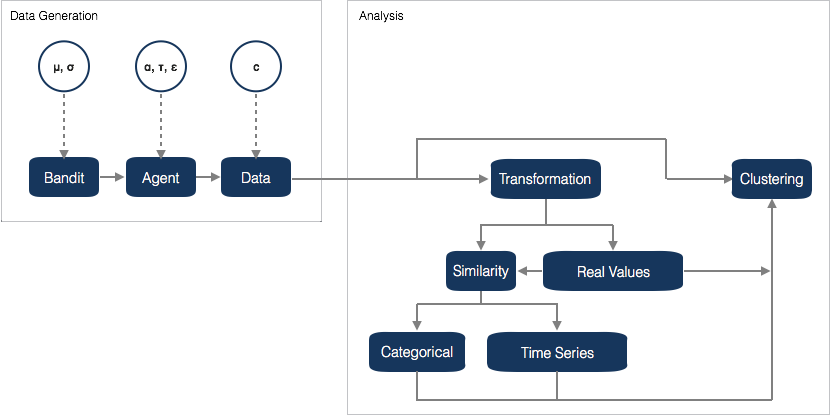
\includegraphics[width=\textwidth]{Pictures/flow01.png}
	\caption{Flowchart experiment design}
	\label{fig:flow}
\end{figure}

\subsection{Reinforcement Learning background and multi arm bandits}
\label{reinf}
Our simulation requires an artificial agent to produce desired data. The agent is relying \textit{Reinforcement Learning} (RL). Thus, we provide some necessary concepts of that field. The following definitions coming from \cite[chapter 1 and 2]{Sutton2012}. RL is a branch of \textit{machine learning} trying model the interaction of an artificial agents with its environment and the corresponding learning process. \\
In our particular setting the agent is confronted with the task of choosing sequentially from a set of possible choices. The agent doesn't have any knowledge about the system a priori. Therefore, it has to learn the nature of the system by continuously interacting with its environment while keeping track of the obtained information for each particular choice. Due to the lack of examples it has to explore different possible actions to identify the best action. Hence, it is useful to deviate from the current optimal strategy from time to time.\\ 
Each action in each step is associated with a given value based on the experience of the agent. This is modeled by defining a value function value function each action $a$. Denote the value function of an action $a$ as $Q_t(a)$ and define it as:
\begin{flalign}
Q_t(a) := \frac{R_1 + R_2 + \dots + R_{K_\alpha}}{K_\alpha} 
\label{eq:valuefunction}
\end{flalign}
where $R$ denotes rewards. Hence the value function is defined average over the rewards for a given state [COMMENT - REFORMULATE THIS]. As mentioned it is necessary for the agent to explore its environment while simultaneously try to optimize its utility. Thus, a crucial task of the agent is to balance \textit{exploration} and \textit{exploitation} of the environment. There are two basic approaches to model this trade-off; An \textit{"Epsilon-Greedy"} action selection method and \textit{"Softmax"} selection method.\\
Within an epsilon greedy action selection strategy the next action is chosen based on the highest value function. However, to model exploration an random element is introduced to deviate from that greedy strategy with a certain probability (denoted by $\epsilon$). In general we can define the next action selected by the epsilon greedy strategy as:
\begin{flalign}
a_{t+1} = \begin{cases} 
\text{random action} & \text{, with probability } \epsilon \\
\arg \max_i Q_t(i) & \text{, with probability } 1-\epsilon
\end{cases} \nonumber
\end{flalign}
In the softmax action selection method each next action is sampled with a certain probability coming from a  \textit{Boltzmann Distribution)}. The probability for action a is computed by:
\begin{flalign}
P(a_{t}) = \frac{e^{\frac{Q_t(a)}{\tau}}}{\sum_{i}^{K} e^{\frac{Q_t(i)}{\tau}}}
\label{eq:softmax}
\end{flalign}
By computing this probability for each action the next action is sampled using those probabilities. The softmax is essentially depending on the parameter $\tau$ functions. It is controlling the how deterministic or random the agent is behaving. For increasing $\tau$ the numerator goes to one and the next action is therefore picked uniformly. For low values in $\tau$, actions with low value functions result in lower probabilities and hence in a greedy strategy. The parameter is also sometimes called \textit{temparature}.\footnote{Sometimes another variation to use the inverse of tau. Obviously that would flip those intuitions.} Finally the next action gets sample from a distribution with the probabilities obtained by equation \eqref{eq:softmax}.
\begin{flalign}
a_{t+1} \sim p_a \nonumber
\end{flalign}
After selecting an action the agent has to update its believe of the chosen action. One can show that equation \eqref{eq:valuefunction} can be expressed in the following way: [THIS HAS TO BE CHANGED - MISLEADING]
\begin{flalign}
Q(a)_{k+1} = Q(a)_k + \alpha \left[ R(a)_k -  Q(a)_k	 \right], 
\label{eq:update}
\end{flalign}
where $\alpha$ is a is the non negative \textit{learning rate} defining how much the current action is affecting the believes. A challange might be how to initialize the value function. However, for convenience we set them to zero for all bandits. Those are the basic necessary ingredients to model artificial decision process. In the following we elaborate on further data processing.

\subsection{Data handling, unsupervised learning methods and similarities}
\label{algosim}
As mentioned we find two main challenges concerning the data. First, our data have a categorical nature. Furthermore, the learning process and corresponding behavioural changes also imposes changing dependence over time.\\
A well studied approach clustering such data types are \textit{hidden markov models}. For example, a decent study on that can be found in \cite{Pamminger2007}, \cite{Pamminger2009} and \cite{Pamminger2010a}. However, we focus our attention only on partition based clustering algorithms.\\
Some of the applied algorithms operate on distinct distance or similarity concepts. Given our data we  have to think carefully think about distance and similarity measures to respect the nature of our data and algorithms.\footnote{A formal definition of the distance and similarity can be found in the appendix} 
Furthermore, besides considering only raw choices we might try to re-express our data to discriminate them in different ways. 
One way is to apply \textit{Shannon's Entropy}  introduced by \cite{Shannon1948}. It is computed by using the empirical probability for each choices. For a discrete random variable  $X$ with probability $p$ the entropy is defined as \cite[page 32]{MacKay2005}:
\begin{flalign}
H(X) := -\sum_{i=1}^{N} p_i \log_2 p_i
\end{flalign}
Entropy gives measure on how random a random variable behaves.\footnote{In case we get a value for X such that $p_i = 0$, we set $H(X) = 0$  \cite[page 49]{Bishop2006}} Within the entropy framework we consider to types of entropies. For each time step we compute the entropy using choices done so far. We call this \textit{cumulative entropy}. Furthermore, we might want to observe more clearly how individuals adapt their behaviour over time. Considering an experiment with 100 trials we then compute the entropy for set of e.g. ten choices. We call this \textit{blockwise entropy}. Mapping choices to an entropy data set aims on discriminating individuals by their level randomness in their behaviour. \\
A second approach is based on the experimental setting. We know that within framework there are a set of choices, which are disadvantageous for the participant. Following e.g. \cite{Yechiam2008} or \cite{Ahn2008}, we then compute block wise the ratio of disadvantageous choices. We call this \textit{blockwise disadvantageous choice}. 

Within our analysis we consider a broad selection of several clustering techniques and similarity concepts. Figure \ref{fig:cla} shows an overview of the algorithms and their corresponding distance/similarity requirements. A technical description for all of them is provided in the appendix. 
\begin{figure}[H]
	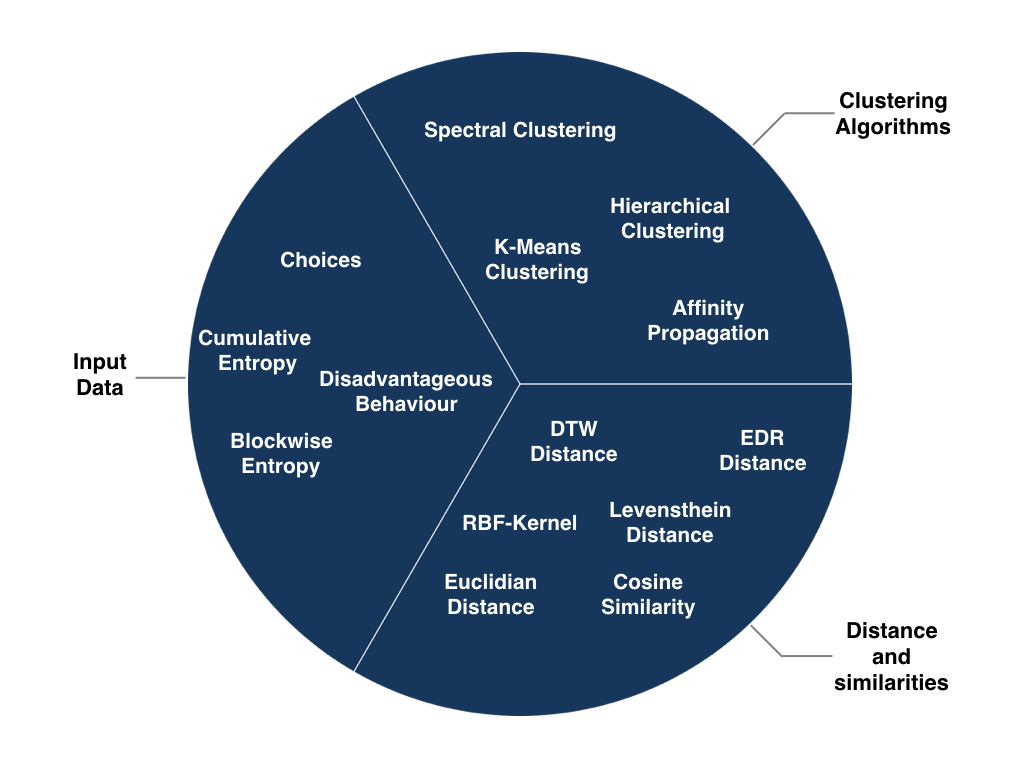
\includegraphics[width=\textwidth]{Pictures/DataClustering.jpeg}
	\caption{Input data, algorithms and proximity measures}
	\label{fig:cla}
\end{figure}

\subsection{Simulation setup and results}

We observed that that the clustering results of our simulation are fluctuating. Hence, to report stable results, the following numbers are computed as an average for each settings over 20 simulations. We also report the corresponding standard deviations to give an impression on the sensitivity of the clustering.\\
Our implementation is quite flexible. We can control both all parameters for each individual agent and their reward sets. We can control the number of trials for each agent and produce customized and multiple asymmetric cluster sizes. Furthermore, we can set prior values for each agent and each value function for the bandits. However, within our experiment we kept the settings simple. First we fix means and standard deviations for the bandits. Then first fix a value for alpha and run the simulations for different differences in tau. We repeat this procedure for fixed values of tau and vary alpha. Finally, we repeat this procedure with a different setting in the bandit means.\\
We are confronted with an enormous grid search over different parameters. Computing distances is very costly. As mentioned we have to run our simulations multiple times to get an impression of the variability. To keep the computation time to a reasonable we let them perform 100 trials and set the number to 10 for each parameter setting. We ended up using solely the softmax function. The main reason for that decision is that we estimate those parameters later on for the experimental data.\\ 
The following table shows a snippet of our simulation results. As described in the last section we have a broad range o similarity measures and algorithms. Therefore, we selected results in such a way, that we give an impression when clustering is working well. Naturally we also found a lot of settings where clustering was not successful. A detailed overview on the numbers are given by tables \ref{tab:apstab1} to \ref{tab:apstab8} in the appendix.\footnote{To give an intuition about the numbers one can informally note that numbers below 0.200 - 0.300 do not show any really good clustering patterns.}

%---------------------------------------------------------------------------------------------------------
% 4. Data
%---------------------------------------------------------------------------------------------------------

\section{Data Analysis}

Our simulation results suggested that we can cluster the decision behaviour under some given constraints. In the following we apply our methods to three different real experiment data. The first data comes  As mentioned in the introduction the Iowa gambling task is popular way to monitor decision and learning process of individuals. s
In the simulation setting we initially define participants with a certain set of parameters. There exist techniques to estimate those parameters from actual data. 

\subsection{Multi-arm bandit experiment data}

The first data set is related to \cite{Stojic2015}. The data are gathered in a 20-arm bandits online experiment, in which users were compensated with small amount of money in exchange. Four different distributional settings were given to different people. In total the data sets consists of 429 participants divided in 199 female and 229 male participants.\footnote{One did not wish to answer} The average age 33.04 with standard deviation 11.75. Furthermore, the participants overall have a stronger higher education background. 261 participants have college degree, 39 a graduate degree and PhD respectively. 127 have a high school degree and 2 declined to answer.\\
We tried to identify different clusterings according to those demographics within those four sub experiments. Our results doesn't show worth mentioning clustering across demographics.\\
We try to discover clustering in the data. Within our simulation we set parameters, which classify individual subjects. Using the experimental data we come from the other way. The reinforcement learning model is quite closely related to the expectancy valence model from cognitive science. Referring to equation \eqref{eq:softmax} and equation \eqref{eq:update} we can try to recover the parameters by optimising those function based on the observed choices. 

\subsection{Prison data}

We were provided with experimental data from \cite{Yechiam2008}. Again we try to apply our methods to cluster different groups in the data. The participants had to perform a modified version of the Iowa gambling task, where reward structure of the decks are changing over time.\\
In particular we have data of 96 individuals with different criminal profile. Within this data we don't have a control group. Given that participants performed a different version of the test we could add a control data from publicly available data sets (see \cite{Steingroever2015}).\\
Table \ref{tab:tabps} gives a broad summary of some demographics of the participants. The samples for each groups are not balanced. 

\begin{table}[H]
	\scriptsize
	 \centering 
	\resizebox{\textwidth}{!}{\begin{tabular}{ l|ccccc} 
		\toprule 
		Crime & \textbf{Count} & \textbf{Age} & \textbf{TABE Score} & \textbf{Education} & \textbf{Beta IQ} \\ 
		\hline
	Theft/Burglary & $22$ & $25.36$  (7.03) & $11.09$ (1.29) & $7.38$ (3.34 )& $92.91$ (14.37) \\ 
	Robbery & $6$ & $24.17$ (9.83) & $11.00$ (0.63) & $9.22$ (3.30) & $96.50$ (7.58) \\          
	Sex & $17$ & $33.41$ (13.59) & $10.97$ (1.47) & $9.15$ (2.98) & $99.65$ (11.74) \\       
	Drug & $22$ & $30.91$ (10.11)  & $11.64$ (1.85)& $9.06$   (2.70)  & $100.36$ (12.92) \\     
	OWI & $4$ & $38.75$ (7.27) & $10.88$ (1.93) & $7.12$ (1.17)& $94.25$ (10.40) \\        
	Assault & $10$ & $27.20$ (8.77) & $12.30$ (2.41)& $7.62$ (2.28) & $94.50$ (11.29) \\       
	Escape/ Failure To Appear & $4$ & $2.008$ (5.60)& $11.00$ (1.35)& $7.78$  (3.21)& $96.50$  (14.18)\\     
	Vandalism & $1$ & $18.00$ (NA)& $11.00$ (NA)& $9.40$ (NA)& $90.00$ (NA)\\ 
	Forgery & $7$ & $34.57$ (13.14)& $10.93$ (5.15) & $9.83$ (3.82)& $100.71$ (11.01)\\       
	Probabiton & $1$ & $38.00$ (NA)& $12.00$ (NA)& $6.30$ (NA)& $92.00$ (NA)\\ 
	Other & $2$ & $35.00$ (9.90)& $11.50$ (0.00)& $9.20$ (4.67)& $95.00$ (5.66)\\       
		\bottomrule 
	\end{tabular} }
		\caption{Summary prison data (means with standard deviation in parenthesis)} 
		\label{tab:tabps} 
\end{table} 

Figure \ref{fig:ent} (a) shows the average cumulative entropy averaged across groups. We observe a random behaviour independent from group affiliation. However, normal people show the least random behaviour. Furthermore, Figure \ref{fig:ent} (b) shows the average people of negative choices people chose over steps of ten periods averaged across groups.     

\setlength{\tabcolsep}{-0.2cm}
\renewcommand{\arraystretch}{-0.6}
\begin{figure}[H]
	\small
	\begin{tabular}{cc}
	% Created by tikzDevice version 0.10.1 on 2016-06-29 16:09:48
% !TEX encoding = UTF-8 Unicode
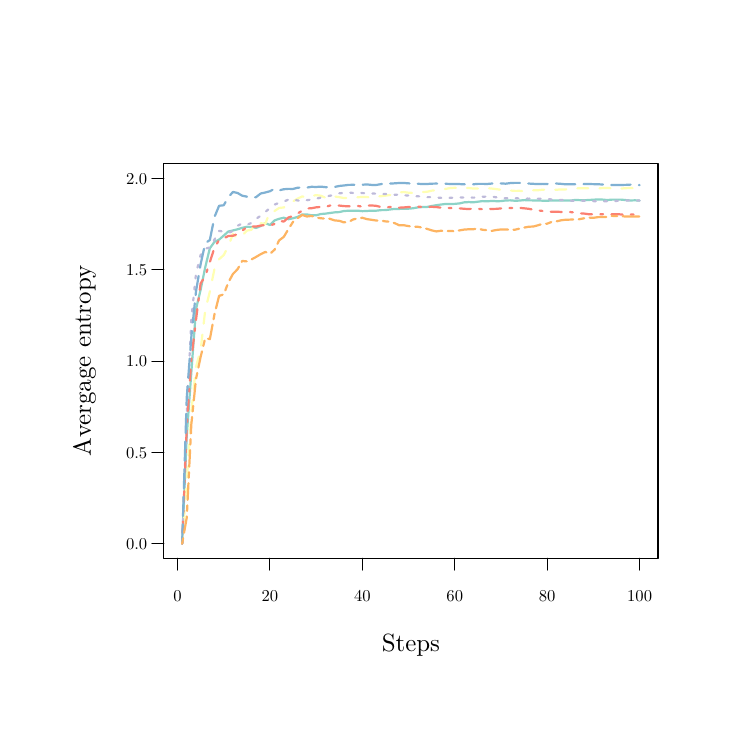
\begin{tikzpicture}[x=1pt,y=1pt]
\definecolor{fillColor}{RGB}{255,255,255}
\path[use as bounding box,fill=fillColor,fill opacity=0.00] (0,0) rectangle (252.94,252.94);
\begin{scope}
\path[clip] ( 49.20, 61.20) rectangle (227.75,203.75);
\definecolor{drawColor}{RGB}{141,211,199}

\path[draw=drawColor,line width= 0.8pt,line join=round,line cap=round] ( 55.81, 66.48) --
	( 57.48,105.48) --
	( 59.15,128.55) --
	( 60.82,151.21) --
	( 62.49,158.21) --
	( 64.16,166.36) --
	( 65.83,173.24) --
	( 67.50,175.53) --
	( 69.17,176.36) --
	( 70.84,177.80) --
	( 72.51,179.29) --
	( 74.18,179.66) --
	( 75.85,180.08) --
	( 77.52,180.61) --
	( 79.19,180.97) --
	( 80.86,180.93) --
	( 82.53,180.57) --
	( 84.20,181.25) --
	( 85.87,182.30) --
	( 87.54,181.63) --
	( 89.21,183.28) --
	( 90.88,183.88) --
	( 92.55,184.25) --
	( 94.22,183.73) --
	( 95.89,184.07) --
	( 97.56,184.57) --
	( 99.23,185.45) --
	(100.90,185.44) --
	(102.57,185.15) --
	(104.24,185.14) --
	(105.91,185.60) --
	(107.58,185.74) --
	(109.25,185.97) --
	(110.92,186.20) --
	(112.59,186.30) --
	(114.26,186.69) --
	(115.93,186.78) --
	(117.60,186.80) --
	(119.27,186.81) --
	(120.94,186.63) --
	(122.61,186.71) --
	(124.28,186.81) --
	(125.95,186.81) --
	(127.62,187.00) --
	(129.29,187.02) --
	(130.96,187.24) --
	(132.63,187.45) --
	(134.30,187.45) --
	(135.97,187.49) --
	(137.64,187.54) --
	(139.31,187.69) --
	(140.98,187.99) --
	(142.65,188.12) --
	(144.32,188.15) --
	(145.99,188.49) --
	(147.66,188.79) --
	(149.33,189.03) --
	(151.00,189.23) --
	(152.67,189.20) --
	(154.34,189.27) --
	(156.01,189.43) --
	(157.68,189.81) --
	(159.35,189.92) --
	(161.02,189.83) --
	(162.69,190.05) --
	(164.36,190.27) --
	(166.03,190.19) --
	(167.70,190.32) --
	(169.37,190.24) --
	(171.04,190.26) --
	(172.71,190.50) --
	(174.38,190.54) --
	(176.05,190.40) --
	(177.71,190.45) --
	(179.38,190.63) --
	(181.05,190.54) --
	(182.72,190.52) --
	(184.39,190.45) --
	(186.06,190.43) --
	(187.73,190.40) --
	(189.40,190.48) --
	(191.07,190.48) --
	(192.74,190.50) --
	(194.41,190.52) --
	(196.08,190.45) --
	(197.75,190.68) --
	(199.42,190.62) --
	(201.09,190.57) --
	(202.76,190.68) --
	(204.43,190.77) --
	(206.10,190.89) --
	(207.77,190.81) --
	(209.44,190.65) --
	(211.11,190.80) --
	(212.78,190.80) --
	(214.45,190.80) --
	(216.12,190.63) --
	(217.79,190.50) --
	(219.46,190.55) --
	(221.13,190.44);
\end{scope}
\begin{scope}
\path[clip] (  0.00,  0.00) rectangle (252.94,252.94);
\definecolor{drawColor}{RGB}{0,0,0}

\path[draw=drawColor,line width= 0.4pt,line join=round,line cap=round] ( 54.14, 61.20) -- (221.13, 61.20);

\path[draw=drawColor,line width= 0.4pt,line join=round,line cap=round] ( 54.14, 61.20) -- ( 54.14, 56.92);

\path[draw=drawColor,line width= 0.4pt,line join=round,line cap=round] ( 87.54, 61.20) -- ( 87.54, 56.92);

\path[draw=drawColor,line width= 0.4pt,line join=round,line cap=round] (120.94, 61.20) -- (120.94, 56.92);

\path[draw=drawColor,line width= 0.4pt,line join=round,line cap=round] (154.34, 61.20) -- (154.34, 56.92);

\path[draw=drawColor,line width= 0.4pt,line join=round,line cap=round] (187.73, 61.20) -- (187.73, 56.92);

\path[draw=drawColor,line width= 0.4pt,line join=round,line cap=round] (221.13, 61.20) -- (221.13, 56.92);

\node[text=drawColor,anchor=base,inner sep=0pt, outer sep=0pt, scale=  0.60] at ( 54.14, 45.60) {0};

\node[text=drawColor,anchor=base,inner sep=0pt, outer sep=0pt, scale=  0.60] at ( 87.54, 45.60) {20};

\node[text=drawColor,anchor=base,inner sep=0pt, outer sep=0pt, scale=  0.60] at (120.94, 45.60) {40};

\node[text=drawColor,anchor=base,inner sep=0pt, outer sep=0pt, scale=  0.60] at (154.34, 45.60) {60};

\node[text=drawColor,anchor=base,inner sep=0pt, outer sep=0pt, scale=  0.60] at (187.73, 45.60) {80};

\node[text=drawColor,anchor=base,inner sep=0pt, outer sep=0pt, scale=  0.60] at (221.13, 45.60) {100};

\path[draw=drawColor,line width= 0.4pt,line join=round,line cap=round] ( 49.20, 66.48) -- ( 49.20,198.47);

\path[draw=drawColor,line width= 0.4pt,line join=round,line cap=round] ( 49.20, 66.48) -- ( 44.92, 66.48);

\path[draw=drawColor,line width= 0.4pt,line join=round,line cap=round] ( 49.20, 99.48) -- ( 44.92, 99.48);

\path[draw=drawColor,line width= 0.4pt,line join=round,line cap=round] ( 49.20,132.47) -- ( 44.92,132.47);

\path[draw=drawColor,line width= 0.4pt,line join=round,line cap=round] ( 49.20,165.47) -- ( 44.92,165.47);

\path[draw=drawColor,line width= 0.4pt,line join=round,line cap=round] ( 49.20,198.47) -- ( 44.92,198.47);

\node[text=drawColor,anchor=base east,inner sep=0pt, outer sep=0pt, scale=  0.60] at ( 43.20, 64.41) {0.0};

\node[text=drawColor,anchor=base east,inner sep=0pt, outer sep=0pt, scale=  0.60] at ( 43.20, 97.41) {0.5};

\node[text=drawColor,anchor=base east,inner sep=0pt, outer sep=0pt, scale=  0.60] at ( 43.20,130.41) {1.0};

\node[text=drawColor,anchor=base east,inner sep=0pt, outer sep=0pt, scale=  0.60] at ( 43.20,163.40) {1.5};

\node[text=drawColor,anchor=base east,inner sep=0pt, outer sep=0pt, scale=  0.60] at ( 43.20,196.40) {2.0};

\path[draw=drawColor,line width= 0.4pt,line join=round,line cap=round] ( 49.20, 61.20) --
	(227.75, 61.20) --
	(227.75,203.75) --
	( 49.20,203.75) --
	( 49.20, 61.20);
\end{scope}
\begin{scope}
\path[clip] (  0.00,  0.00) rectangle (252.94,252.94);
\definecolor{drawColor}{RGB}{0,0,0}

\node[text=drawColor,anchor=base,inner sep=0pt, outer sep=0pt, scale=  0.90] at (138.47, 27.60) {Steps};

\node[text=drawColor,rotate= 90.00,anchor=base,inner sep=0pt, outer sep=0pt, scale=  0.90] at ( 22.80,132.47) {Avergage entropy};
\end{scope}
\begin{scope}
\path[clip] ( 49.20, 61.20) rectangle (227.75,203.75);
\definecolor{drawColor}{RGB}{255,255,179}

\path[draw=drawColor,line width= 0.8pt,dash pattern=on 4pt off 4pt ,line join=round,line cap=round] ( 55.81, 66.48) --
	( 57.48, 88.48) --
	( 59.15,114.21) --
	( 60.82,130.40) --
	( 62.49,136.40) --
	( 64.16,150.88) --
	( 65.83,157.60) --
	( 67.50,165.78) --
	( 69.17,169.28) --
	( 70.84,170.76) --
	( 72.51,173.95) --
	( 74.18,178.42) --
	( 75.85,176.74) --
	( 77.52,177.76) --
	( 79.19,179.60) --
	( 80.86,179.90) --
	( 82.53,182.58) --
	( 84.20,182.27) --
	( 85.87,182.08) --
	( 87.54,186.41) --
	( 89.21,186.68) --
	( 90.88,187.80) --
	( 92.55,187.97) --
	( 94.22,189.39) --
	( 95.89,190.17) --
	( 97.56,191.18) --
	( 99.23,191.95) --
	(100.90,191.57) --
	(102.57,192.08) --
	(104.24,192.43) --
	(105.91,192.22) --
	(107.58,191.49) --
	(109.25,192.16) --
	(110.92,191.93) --
	(112.59,191.69) --
	(114.26,191.36) --
	(115.93,191.42) --
	(117.60,191.47) --
	(119.27,191.66) --
	(120.94,191.77) --
	(122.61,191.72) --
	(124.28,191.60) --
	(125.95,191.98) --
	(127.62,192.03) --
	(129.29,192.24) --
	(130.96,192.46) --
	(132.63,192.98) --
	(134.30,193.45) --
	(135.97,193.53) --
	(137.64,193.30) --
	(139.31,193.22) --
	(140.98,193.25) --
	(142.65,193.53) --
	(144.32,193.64) --
	(145.99,194.04) --
	(147.66,194.22) --
	(149.33,194.47) --
	(151.00,194.68) --
	(152.67,194.98) --
	(154.34,195.08) --
	(156.01,195.04) --
	(157.68,195.02) --
	(159.35,195.01) --
	(161.02,194.80) --
	(162.69,194.79) --
	(164.36,194.89) --
	(166.03,194.95) --
	(167.70,194.80) --
	(169.37,194.60) --
	(171.04,194.35) --
	(172.71,194.20) --
	(174.38,194.10) --
	(176.05,193.96) --
	(177.71,193.98) --
	(179.38,193.84) --
	(181.05,193.95) --
	(182.72,194.17) --
	(184.39,194.19) --
	(186.06,194.40) --
	(187.73,194.37) --
	(189.40,194.36) --
	(191.07,194.37) --
	(192.74,194.49) --
	(194.41,194.50) --
	(196.08,194.65) --
	(197.75,194.89) --
	(199.42,194.88) --
	(201.09,194.92) --
	(202.76,194.92) --
	(204.43,194.82) --
	(206.10,194.90) --
	(207.77,194.97) --
	(209.44,195.05) --
	(211.11,194.89) --
	(212.78,194.83) --
	(214.45,194.81) --
	(216.12,194.94) --
	(217.79,195.00) --
	(219.46,194.93) --
	(221.13,194.78);
\definecolor{drawColor}{RGB}{190,186,218}

\path[draw=drawColor,line width= 0.8pt,dash pattern=on 1pt off 3pt ,line join=round,line cap=round] ( 55.81, 66.48) --
	( 57.48,113.06) --
	( 59.15,147.78) --
	( 60.82,164.00) --
	( 62.49,170.78) --
	( 64.16,173.09) --
	( 65.83,173.52) --
	( 67.50,176.37) --
	( 69.17,179.51) --
	( 70.84,179.25) --
	( 72.51,178.77) --
	( 74.18,179.49) --
	( 75.85,181.38) --
	( 77.52,182.16) --
	( 79.19,181.72) --
	( 80.86,182.36) --
	( 82.53,183.89) --
	( 84.20,184.96) --
	( 85.87,186.39) --
	( 87.54,187.71) --
	( 89.21,189.00) --
	( 90.88,189.68) --
	( 92.55,190.11) --
	( 94.22,190.81) --
	( 95.89,190.76) --
	( 97.56,190.51) --
	( 99.23,190.15) --
	(100.90,190.60) --
	(102.57,190.82) --
	(104.24,191.15) --
	(105.91,191.51) --
	(107.58,191.94) --
	(109.25,192.21) --
	(110.92,192.60) --
	(112.59,193.07) --
	(114.26,193.23) --
	(115.93,193.35) --
	(117.60,193.22) --
	(119.27,193.35) --
	(120.94,193.16) --
	(122.61,193.11) --
	(124.28,193.03) --
	(125.95,192.95) --
	(127.62,192.78) --
	(129.29,192.85) --
	(130.96,192.72) --
	(132.63,192.54) --
	(134.30,192.65) --
	(135.97,192.37) --
	(137.64,192.29) --
	(139.31,192.06) --
	(140.98,192.00) --
	(142.65,191.90) --
	(144.32,191.70) --
	(145.99,191.70) --
	(147.66,191.58) --
	(149.33,191.45) --
	(151.00,191.25) --
	(152.67,191.46) --
	(154.34,191.57) --
	(156.01,191.64) --
	(157.68,191.53) --
	(159.35,191.58) --
	(161.02,191.52) --
	(162.69,191.58) --
	(164.36,191.86) --
	(166.03,191.90) --
	(167.70,191.89) --
	(169.37,191.64) --
	(171.04,191.40) --
	(172.71,191.31) --
	(174.38,191.38) --
	(176.05,191.28) --
	(177.71,191.25) --
	(179.38,191.21) --
	(181.05,191.16) --
	(182.72,191.23) --
	(184.39,191.16) --
	(186.06,191.13) --
	(187.73,191.04) --
	(189.40,190.85) --
	(191.07,190.69) --
	(192.74,190.70) --
	(194.41,190.60) --
	(196.08,190.40) --
	(197.75,190.34) --
	(199.42,190.46) --
	(201.09,190.40) --
	(202.76,190.33) --
	(204.43,190.26) --
	(206.10,190.18) --
	(207.77,190.16) --
	(209.44,190.20) --
	(211.11,190.27) --
	(212.78,190.34) --
	(214.45,190.42) --
	(216.12,190.46) --
	(217.79,190.51) --
	(219.46,190.51) --
	(221.13,190.45);
\definecolor{drawColor}{RGB}{251,128,114}

\path[draw=drawColor,line width= 0.8pt,dash pattern=on 1pt off 3pt on 4pt off 3pt ,line join=round,line cap=round] ( 55.81, 66.48) --
	( 57.48,108.48) --
	( 59.15,133.31) --
	( 60.82,147.27) --
	( 62.49,160.54) --
	( 64.16,163.12) --
	( 65.83,168.26) --
	( 67.50,173.44) --
	( 69.17,176.21) --
	( 70.84,176.78) --
	( 72.51,177.68) --
	( 74.18,177.74) --
	( 75.85,178.36) --
	( 77.52,179.52) --
	( 79.19,180.95) --
	( 80.86,181.06) --
	( 82.53,181.06) --
	( 84.20,181.44) --
	( 85.87,181.61) --
	( 87.54,181.42) --
	( 89.21,182.03) --
	( 90.88,183.13) --
	( 92.55,182.88) --
	( 94.22,184.34) --
	( 95.89,184.93) --
	( 97.56,185.80) --
	( 99.23,186.84) --
	(100.90,187.60) --
	(102.57,187.69) --
	(104.24,188.02) --
	(105.91,188.16) --
	(107.58,188.17) --
	(109.25,188.66) --
	(110.92,188.48) --
	(112.59,188.65) --
	(114.26,188.47) --
	(115.93,188.38) --
	(117.60,188.54) --
	(119.27,188.52) --
	(120.94,188.27) --
	(122.61,188.64) --
	(124.28,188.70) --
	(125.95,188.55) --
	(127.62,188.14) --
	(129.29,188.01) --
	(130.96,188.14) --
	(132.63,188.25) --
	(134.30,187.90) --
	(135.97,187.98) --
	(137.64,188.14) --
	(139.31,188.16) --
	(140.98,188.26) --
	(142.65,188.18) --
	(144.32,188.14) --
	(145.99,188.20) --
	(147.66,188.12) --
	(149.33,187.88) --
	(151.00,187.84) --
	(152.67,187.79) --
	(154.34,187.67) --
	(156.01,187.66) --
	(157.68,187.50) --
	(159.35,187.39) --
	(161.02,187.56) --
	(162.69,187.49) --
	(164.36,187.34) --
	(166.03,187.43) --
	(167.70,187.43) --
	(169.37,187.47) --
	(171.04,187.63) --
	(172.71,187.71) --
	(174.38,187.75) --
	(176.05,187.80) --
	(177.71,187.82) --
	(179.38,187.67) --
	(181.05,187.48) --
	(182.72,187.19) --
	(184.39,186.92) --
	(186.06,186.71) --
	(187.73,186.51) --
	(189.40,186.40) --
	(191.07,186.45) --
	(192.74,186.34) --
	(194.41,186.40) --
	(196.08,186.31) --
	(197.75,186.16) --
	(199.42,185.87) --
	(201.09,185.76) --
	(202.76,185.53) --
	(204.43,185.49) --
	(206.10,185.54) --
	(207.77,185.55) --
	(209.44,185.42) --
	(211.11,185.50) --
	(212.78,185.55) --
	(214.45,185.45) --
	(216.12,185.39) --
	(217.79,185.39) --
	(219.46,185.50) --
	(221.13,185.49);
\definecolor{drawColor}{RGB}{128,177,211}

\path[draw=drawColor,line width= 0.8pt,dash pattern=on 7pt off 3pt ,line join=round,line cap=round] ( 55.81, 66.48) --
	( 57.48,119.27) --
	( 59.15,141.36) --
	( 60.82,157.62) --
	( 62.49,167.43) --
	( 64.16,175.07) --
	( 65.83,176.19) --
	( 67.50,184.53) --
	( 69.17,188.58) --
	( 70.84,188.76) --
	( 72.51,191.69) --
	( 74.18,193.58) --
	( 75.85,193.20) --
	( 77.52,192.22) --
	( 79.19,191.88) --
	( 80.86,191.35) --
	( 82.53,191.70) --
	( 84.20,193.02) --
	( 85.87,193.38) --
	( 87.54,193.84) --
	( 89.21,194.74) --
	( 90.88,194.15) --
	( 92.55,194.56) --
	( 94.22,194.69) --
	( 95.89,194.66) --
	( 97.56,195.11) --
	( 99.23,195.19) --
	(100.90,195.16) --
	(102.57,195.44) --
	(104.24,195.37) --
	(105.91,195.50) --
	(107.58,195.31) --
	(109.25,195.30) --
	(110.92,195.38) --
	(112.59,195.74) --
	(114.26,195.91) --
	(115.93,196.13) --
	(117.60,196.15) --
	(119.27,196.24) --
	(120.94,196.19) --
	(122.61,196.28) --
	(124.28,196.12) --
	(125.95,196.10) --
	(127.62,196.39) --
	(129.29,196.66) --
	(130.96,196.60) --
	(132.63,196.69) --
	(134.30,196.82) --
	(135.97,196.82) --
	(137.64,196.68) --
	(139.31,196.58) --
	(140.98,196.53) --
	(142.65,196.44) --
	(144.32,196.45) --
	(145.99,196.57) --
	(147.66,196.60) --
	(149.33,196.60) --
	(151.00,196.52) --
	(152.67,196.47) --
	(154.34,196.48) --
	(156.01,196.42) --
	(157.68,196.33) --
	(159.35,196.47) --
	(161.02,196.35) --
	(162.69,196.50) --
	(164.36,196.50) --
	(166.03,196.46) --
	(167.70,196.61) --
	(169.37,196.75) --
	(171.04,196.67) --
	(172.71,196.56) --
	(174.38,196.78) --
	(176.05,196.86) --
	(177.71,196.86) --
	(179.38,196.73) --
	(181.05,196.61) --
	(182.72,196.51) --
	(184.39,196.41) --
	(186.06,196.49) --
	(187.73,196.45) --
	(189.40,196.58) --
	(191.07,196.61) --
	(192.74,196.50) --
	(194.41,196.33) --
	(196.08,196.34) --
	(197.75,196.33) --
	(199.42,196.37) --
	(201.09,196.45) --
	(202.76,196.43) --
	(204.43,196.40) --
	(206.10,196.35) --
	(207.77,196.27) --
	(209.44,196.18) --
	(211.11,196.06) --
	(212.78,196.06) --
	(214.45,196.12) --
	(216.12,196.13) --
	(217.79,196.22) --
	(219.46,196.15) --
	(221.13,196.05);
\definecolor{drawColor}{RGB}{253,180,98}

\path[draw=drawColor,line width= 0.8pt,dash pattern=on 2pt off 2pt on 6pt off 2pt ,line join=round,line cap=round] ( 55.81, 66.48) --
	( 57.48, 75.91) --
	( 59.15,109.77) --
	( 60.82,125.98) --
	( 62.49,133.95) --
	( 64.16,140.78) --
	( 65.83,140.38) --
	( 67.50,149.34) --
	( 69.17,156.03) --
	( 70.84,156.54) --
	( 72.51,160.88) --
	( 74.18,163.96) --
	( 75.85,165.66) --
	( 77.52,168.64) --
	( 79.19,168.48) --
	( 80.86,169.18) --
	( 82.53,170.09) --
	( 84.20,171.09) --
	( 85.87,171.89) --
	( 87.54,171.19) --
	( 89.21,172.71) --
	( 90.88,176.09) --
	( 92.55,177.34) --
	( 94.22,180.16) --
	( 95.89,182.78) --
	( 97.56,184.12) --
	( 99.23,185.26) --
	(100.90,184.70) --
	(102.57,184.91) --
	(104.24,184.34) --
	(105.91,184.06) --
	(107.58,183.95) --
	(109.25,183.86) --
	(110.92,183.30) --
	(112.59,183.14) --
	(114.26,182.58) --
	(115.93,182.72) --
	(117.60,183.63) --
	(119.27,184.04) --
	(120.94,184.24) --
	(122.61,183.75) --
	(124.28,183.51) --
	(125.95,183.25) --
	(127.62,183.23) --
	(129.29,182.94) --
	(130.96,182.80) --
	(132.63,182.30) --
	(134.30,181.51) --
	(135.97,181.54) --
	(137.64,181.23) --
	(139.31,181.06) --
	(140.98,180.99) --
	(142.65,180.67) --
	(144.32,180.23) --
	(145.99,179.70) --
	(147.66,179.31) --
	(149.33,179.55) --
	(151.00,179.41) --
	(152.67,179.50) --
	(154.34,179.37) --
	(156.01,179.67) --
	(157.68,179.97) --
	(159.35,180.09) --
	(161.02,180.10) --
	(162.69,180.39) --
	(164.36,179.90) --
	(166.03,179.75) --
	(167.70,179.50) --
	(169.37,179.83) --
	(171.04,180.03) --
	(172.71,180.03) --
	(174.38,179.90) --
	(176.05,179.92) --
	(177.71,180.32) --
	(179.38,180.69) --
	(181.05,181.01) --
	(182.72,181.08) --
	(184.39,181.53) --
	(186.06,182.06) --
	(187.73,182.12) --
	(189.40,182.76) --
	(191.07,182.95) --
	(192.74,183.33) --
	(194.41,183.54) --
	(196.08,183.58) --
	(197.75,183.70) --
	(199.42,183.75) --
	(201.09,184.06) --
	(202.76,184.31) --
	(204.43,184.24) --
	(206.10,184.47) --
	(207.77,184.53) --
	(209.44,184.52) --
	(211.11,184.94) --
	(212.78,184.85) --
	(214.45,184.83) --
	(216.12,184.70) --
	(217.79,184.69) --
	(219.46,184.71) --
	(221.13,184.74);
\end{scope}
\end{tikzpicture}
 & % Created by tikzDevice version 0.10.1 on 2016-06-29 15:59:44
% !TEX encoding = UTF-8 Unicode
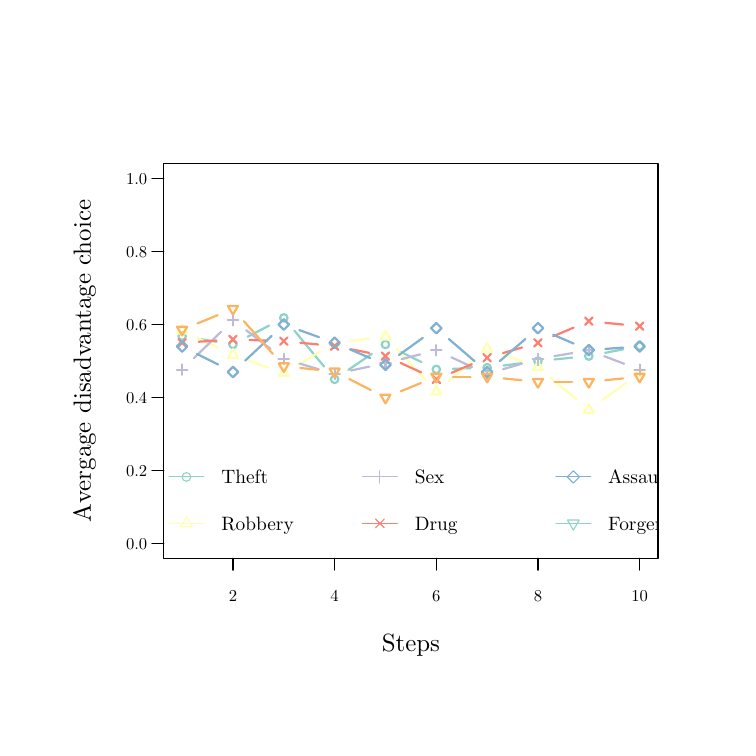
\begin{tikzpicture}[x=1pt,y=1pt]
\definecolor{fillColor}{RGB}{255,255,255}
\path[use as bounding box,fill=fillColor,fill opacity=0.00] (0,0) rectangle (252.94,252.94);
\begin{scope}
\path[clip] ( 49.20, 61.20) rectangle (227.75,203.75);
\definecolor{drawColor}{RGB}{141,211,199}

\path[draw=drawColor,line width= 0.8pt,line join=round,line cap=round] ( 61.73,140.50) -- ( 68.26,139.44);

\path[draw=drawColor,line width= 0.8pt,line join=round,line cap=round] ( 79.50,141.25) -- ( 87.23,145.29);

\path[draw=drawColor,line width= 0.8pt,line join=round,line cap=round] ( 96.38,143.45) -- (107.09,130.50);

\path[draw=drawColor,line width= 0.8pt,line join=round,line cap=round] (115.87,129.27) -- (124.34,135.08);

\path[draw=drawColor,line width= 0.8pt,line join=round,line cap=round] (134.68,135.83) -- (142.27,132.11);

\path[draw=drawColor,line width= 0.8pt,line join=round,line cap=round] (153.65,129.67) -- (160.03,129.88);

\path[draw=drawColor,line width= 0.8pt,line join=round,line cap=round] (171.98,130.85) -- (178.45,131.70);

\path[draw=drawColor,line width= 0.8pt,line join=round,line cap=round] (190.37,133.06) -- (196.79,133.69);

\path[draw=drawColor,line width= 0.8pt,line join=round,line cap=round] (208.65,135.43) -- (215.24,136.72);

\path[draw=drawColor,line width= 0.8pt,line join=round,line cap=round] ( 55.81,141.47) circle (  1.35);

\path[draw=drawColor,line width= 0.8pt,line join=round,line cap=round] ( 74.18,138.47) circle (  1.35);

\path[draw=drawColor,line width= 0.8pt,line join=round,line cap=round] ( 92.55,148.07) circle (  1.35);

\path[draw=drawColor,line width= 0.8pt,line join=round,line cap=round] (110.92,125.87) circle (  1.35);

\path[draw=drawColor,line width= 0.8pt,line join=round,line cap=round] (129.29,138.47) circle (  1.35);

\path[draw=drawColor,line width= 0.8pt,line join=round,line cap=round] (147.66,129.47) circle (  1.35);

\path[draw=drawColor,line width= 0.8pt,line join=round,line cap=round] (166.03,130.07) circle (  1.35);

\path[draw=drawColor,line width= 0.8pt,line join=round,line cap=round] (184.39,132.47) circle (  1.35);

\path[draw=drawColor,line width= 0.8pt,line join=round,line cap=round] (202.76,134.27) circle (  1.35);

\path[draw=drawColor,line width= 0.8pt,line join=round,line cap=round] (221.13,137.87) circle (  1.35);
\end{scope}
\begin{scope}
\path[clip] (  0.00,  0.00) rectangle (252.94,252.94);
\definecolor{drawColor}{RGB}{0,0,0}

\path[draw=drawColor,line width= 0.4pt,line join=round,line cap=round] ( 74.18, 61.20) -- (221.13, 61.20);

\path[draw=drawColor,line width= 0.4pt,line join=round,line cap=round] ( 74.18, 61.20) -- ( 74.18, 56.92);

\path[draw=drawColor,line width= 0.4pt,line join=round,line cap=round] (110.92, 61.20) -- (110.92, 56.92);

\path[draw=drawColor,line width= 0.4pt,line join=round,line cap=round] (147.66, 61.20) -- (147.66, 56.92);

\path[draw=drawColor,line width= 0.4pt,line join=round,line cap=round] (184.39, 61.20) -- (184.39, 56.92);

\path[draw=drawColor,line width= 0.4pt,line join=round,line cap=round] (221.13, 61.20) -- (221.13, 56.92);

\node[text=drawColor,anchor=base,inner sep=0pt, outer sep=0pt, scale=  0.60] at ( 74.18, 45.60) {2};

\node[text=drawColor,anchor=base,inner sep=0pt, outer sep=0pt, scale=  0.60] at (110.92, 45.60) {4};

\node[text=drawColor,anchor=base,inner sep=0pt, outer sep=0pt, scale=  0.60] at (147.66, 45.60) {6};

\node[text=drawColor,anchor=base,inner sep=0pt, outer sep=0pt, scale=  0.60] at (184.39, 45.60) {8};

\node[text=drawColor,anchor=base,inner sep=0pt, outer sep=0pt, scale=  0.60] at (221.13, 45.60) {10};

\path[draw=drawColor,line width= 0.4pt,line join=round,line cap=round] ( 49.20, 66.48) -- ( 49.20,198.47);

\path[draw=drawColor,line width= 0.4pt,line join=round,line cap=round] ( 49.20, 66.48) -- ( 44.92, 66.48);

\path[draw=drawColor,line width= 0.4pt,line join=round,line cap=round] ( 49.20, 92.88) -- ( 44.92, 92.88);

\path[draw=drawColor,line width= 0.4pt,line join=round,line cap=round] ( 49.20,119.27) -- ( 44.92,119.27);

\path[draw=drawColor,line width= 0.4pt,line join=round,line cap=round] ( 49.20,145.67) -- ( 44.92,145.67);

\path[draw=drawColor,line width= 0.4pt,line join=round,line cap=round] ( 49.20,172.07) -- ( 44.92,172.07);

\path[draw=drawColor,line width= 0.4pt,line join=round,line cap=round] ( 49.20,198.47) -- ( 44.92,198.47);

\node[text=drawColor,anchor=base east,inner sep=0pt, outer sep=0pt, scale=  0.60] at ( 43.20, 64.41) {0.0};

\node[text=drawColor,anchor=base east,inner sep=0pt, outer sep=0pt, scale=  0.60] at ( 43.20, 90.81) {0.2};

\node[text=drawColor,anchor=base east,inner sep=0pt, outer sep=0pt, scale=  0.60] at ( 43.20,117.21) {0.4};

\node[text=drawColor,anchor=base east,inner sep=0pt, outer sep=0pt, scale=  0.60] at ( 43.20,143.60) {0.6};

\node[text=drawColor,anchor=base east,inner sep=0pt, outer sep=0pt, scale=  0.60] at ( 43.20,170.00) {0.8};

\node[text=drawColor,anchor=base east,inner sep=0pt, outer sep=0pt, scale=  0.60] at ( 43.20,196.40) {1.0};

\path[draw=drawColor,line width= 0.4pt,line join=round,line cap=round] ( 49.20, 61.20) --
	(227.75, 61.20) --
	(227.75,203.75) --
	( 49.20,203.75) --
	( 49.20, 61.20);
\end{scope}
\begin{scope}
\path[clip] (  0.00,  0.00) rectangle (252.94,252.94);
\definecolor{drawColor}{RGB}{0,0,0}

\node[text=drawColor,anchor=base,inner sep=0pt, outer sep=0pt, scale=  0.90] at (138.47, 27.60) {Steps};

\node[text=drawColor,rotate= 90.00,anchor=base,inner sep=0pt, outer sep=0pt, scale=  0.90] at ( 22.80,132.47) {Avergage disadvantage choice};
\end{scope}
\begin{scope}
\path[clip] ( 49.20, 61.20) rectangle (227.75,203.75);
\definecolor{drawColor}{RGB}{255,255,179}

\path[draw=drawColor,line width= 0.8pt,line join=round,line cap=round] ( 61.22,140.88) -- ( 68.77,137.26);

\path[draw=drawColor,line width= 0.8pt,line join=round,line cap=round] ( 79.83,132.64) -- ( 86.90,130.10);

\path[draw=drawColor,line width= 0.8pt,line join=round,line cap=round] ( 97.70,131.16) -- (105.77,135.99);

\path[draw=drawColor,line width= 0.8pt,line join=round,line cap=round] (116.88,139.79) -- (123.33,140.56);

\path[draw=drawColor,line width= 0.8pt,line join=round,line cap=round] (133.37,136.87) -- (143.58,125.87);

\path[draw=drawColor,line width= 0.8pt,line join=round,line cap=round] (152.26,125.33) -- (161.43,133.02);

\path[draw=drawColor,line width= 0.8pt,line join=round,line cap=round] (171.67,134.84) -- (178.75,132.30);

\path[draw=drawColor,line width= 0.8pt,line join=round,line cap=round] (188.99,126.42) -- (198.17,118.73);

\path[draw=drawColor,line width= 0.8pt,line join=round,line cap=round] (207.64,118.38) -- (216.26,124.57);

\path[draw=drawColor,line width= 0.8pt,line join=round,line cap=round] ( 55.81,145.57) --
	( 57.63,142.42) --
	( 53.99,142.42) --
	( 55.81,145.57);

\path[draw=drawColor,line width= 0.8pt,line join=round,line cap=round] ( 74.18,136.77) --
	( 76.00,133.62) --
	( 72.36,133.62) --
	( 74.18,136.77);

\path[draw=drawColor,line width= 0.8pt,line join=round,line cap=round] ( 92.55,130.17) --
	( 94.37,127.02) --
	( 90.73,127.02) --
	( 92.55,130.17);

\path[draw=drawColor,line width= 0.8pt,line join=round,line cap=round] (110.92,141.17) --
	(112.74,138.02) --
	(109.10,138.02) --
	(110.92,141.17);

\path[draw=drawColor,line width= 0.8pt,line join=round,line cap=round] (129.29,143.37) --
	(131.11,140.22) --
	(127.47,140.22) --
	(129.29,143.37);

\path[draw=drawColor,line width= 0.8pt,line join=round,line cap=round] (147.66,123.57) --
	(149.48,120.42) --
	(145.84,120.42) --
	(147.66,123.57);

\path[draw=drawColor,line width= 0.8pt,line join=round,line cap=round] (166.03,138.97) --
	(167.84,135.82) --
	(164.21,135.82) --
	(166.03,138.97);

\path[draw=drawColor,line width= 0.8pt,line join=round,line cap=round] (184.39,132.37) --
	(186.21,129.22) --
	(182.58,129.22) --
	(184.39,132.37);

\path[draw=drawColor,line width= 0.8pt,line join=round,line cap=round] (202.76,116.97) --
	(204.58,113.82) --
	(200.95,113.82) --
	(202.76,116.97);

\path[draw=drawColor,line width= 0.8pt,line join=round,line cap=round] (221.13,130.17) --
	(222.95,127.02) --
	(219.31,127.02) --
	(221.13,130.17);
\definecolor{drawColor}{RGB}{190,186,218}

\path[draw=drawColor,line width= 0.8pt,line join=round,line cap=round] ( 60.11,133.55) -- ( 69.88,143.04);

\path[draw=drawColor,line width= 0.8pt,line join=round,line cap=round] ( 78.96,143.59) -- ( 87.78,136.88);

\path[draw=drawColor,line width= 0.8pt,line join=round,line cap=round] ( 98.30,131.55) -- (105.17,129.52);

\path[draw=drawColor,line width= 0.8pt,line join=round,line cap=round] (116.79,129.05) -- (123.42,130.46);

\path[draw=drawColor,line width= 0.8pt,line join=round,line cap=round] (135.10,133.17) -- (141.84,134.88);

\path[draw=drawColor,line width= 0.8pt,line join=round,line cap=round] (153.10,133.82) -- (160.59,130.34);

\path[draw=drawColor,line width= 0.8pt,line join=round,line cap=round] (171.78,129.52) -- (178.64,131.55);

\path[draw=drawColor,line width= 0.8pt,line join=round,line cap=round] (190.31,134.25) -- (196.85,135.35);

\path[draw=drawColor,line width= 0.8pt,line join=round,line cap=round] (208.37,134.22) -- (215.52,131.50);

\path[draw=drawColor,line width= 0.8pt,line join=round,line cap=round] ( 53.90,129.37) -- ( 57.72,129.37);

\path[draw=drawColor,line width= 0.8pt,line join=round,line cap=round] ( 55.81,127.46) -- ( 55.81,131.28);

\path[draw=drawColor,line width= 0.8pt,line join=round,line cap=round] ( 72.27,147.22) -- ( 76.09,147.22);

\path[draw=drawColor,line width= 0.8pt,line join=round,line cap=round] ( 74.18,145.31) -- ( 74.18,149.13);

\path[draw=drawColor,line width= 0.8pt,line join=round,line cap=round] ( 90.64,133.25) -- ( 94.46,133.25);

\path[draw=drawColor,line width= 0.8pt,line join=round,line cap=round] ( 92.55,131.34) -- ( 92.55,135.16);

\path[draw=drawColor,line width= 0.8pt,line join=round,line cap=round] (109.01,127.81) -- (112.83,127.81);

\path[draw=drawColor,line width= 0.8pt,line join=round,line cap=round] (110.92,125.90) -- (110.92,129.72);

\path[draw=drawColor,line width= 0.8pt,line join=round,line cap=round] (127.38,131.70) -- (131.20,131.70);

\path[draw=drawColor,line width= 0.8pt,line join=round,line cap=round] (129.29,129.79) -- (129.29,133.61);

\path[draw=drawColor,line width= 0.8pt,line join=round,line cap=round] (145.75,136.35) -- (149.57,136.35);

\path[draw=drawColor,line width= 0.8pt,line join=round,line cap=round] (147.66,134.45) -- (147.66,138.26);

\path[draw=drawColor,line width= 0.8pt,line join=round,line cap=round] (164.12,127.81) -- (167.93,127.81);

\path[draw=drawColor,line width= 0.8pt,line join=round,line cap=round] (166.03,125.90) -- (166.03,129.72);

\path[draw=drawColor,line width= 0.8pt,line join=round,line cap=round] (182.49,133.25) -- (186.30,133.25);

\path[draw=drawColor,line width= 0.8pt,line join=round,line cap=round] (184.39,131.34) -- (184.39,135.16);

\path[draw=drawColor,line width= 0.8pt,line join=round,line cap=round] (200.85,136.35) -- (204.67,136.35);

\path[draw=drawColor,line width= 0.8pt,line join=round,line cap=round] (202.76,134.45) -- (202.76,138.26);

\path[draw=drawColor,line width= 0.8pt,line join=round,line cap=round] (219.22,129.37) -- (223.04,129.37);

\path[draw=drawColor,line width= 0.8pt,line join=round,line cap=round] (221.13,127.46) -- (221.13,131.28);
\definecolor{drawColor}{RGB}{251,128,114}

\path[draw=drawColor,line width= 0.8pt,line join=round,line cap=round] ( 61.80,139.46) -- ( 68.19,139.88);

\path[draw=drawColor,line width= 0.8pt,line join=round,line cap=round] ( 80.18,140.08) -- ( 86.55,139.87);

\path[draw=drawColor,line width= 0.8pt,line join=round,line cap=round] ( 98.52,139.09) -- (104.95,138.46);

\path[draw=drawColor,line width= 0.8pt,line join=round,line cap=round] (116.81,136.72) -- (123.40,135.43);

\path[draw=drawColor,line width= 0.8pt,line join=round,line cap=round] (134.74,131.78) -- (142.20,128.37);

\path[draw=drawColor,line width= 0.8pt,line join=round,line cap=round] (153.18,128.22) -- (160.50,131.33);

\path[draw=drawColor,line width= 0.8pt,line join=round,line cap=round] (171.78,135.36) -- (178.64,137.38);

\path[draw=drawColor,line width= 0.8pt,line join=round,line cap=round] (189.92,141.42) -- (197.24,144.53);

\path[draw=drawColor,line width= 0.8pt,line join=round,line cap=round] (208.73,146.29) -- (215.16,145.66);

\path[draw=drawColor,line width= 0.8pt,line join=round,line cap=round] ( 54.46,137.72) -- ( 57.16,140.42);

\path[draw=drawColor,line width= 0.8pt,line join=round,line cap=round] ( 54.46,140.42) -- ( 57.16,137.72);

\path[draw=drawColor,line width= 0.8pt,line join=round,line cap=round] ( 72.83,138.92) -- ( 75.53,141.62);

\path[draw=drawColor,line width= 0.8pt,line join=round,line cap=round] ( 72.83,141.62) -- ( 75.53,138.92);

\path[draw=drawColor,line width= 0.8pt,line join=round,line cap=round] ( 91.20,138.32) -- ( 93.90,141.02);

\path[draw=drawColor,line width= 0.8pt,line join=round,line cap=round] ( 91.20,141.02) -- ( 93.90,138.32);

\path[draw=drawColor,line width= 0.8pt,line join=round,line cap=round] (109.57,136.52) -- (112.27,139.22);

\path[draw=drawColor,line width= 0.8pt,line join=round,line cap=round] (109.57,139.22) -- (112.27,136.52);

\path[draw=drawColor,line width= 0.8pt,line join=round,line cap=round] (127.94,132.92) -- (130.64,135.62);

\path[draw=drawColor,line width= 0.8pt,line join=round,line cap=round] (127.94,135.62) -- (130.64,132.92);

\path[draw=drawColor,line width= 0.8pt,line join=round,line cap=round] (146.31,124.52) -- (149.01,127.22);

\path[draw=drawColor,line width= 0.8pt,line join=round,line cap=round] (146.31,127.22) -- (149.01,124.52);

\path[draw=drawColor,line width= 0.8pt,line join=round,line cap=round] (164.68,132.32) -- (167.38,135.02);

\path[draw=drawColor,line width= 0.8pt,line join=round,line cap=round] (164.68,135.02) -- (167.38,132.32);

\path[draw=drawColor,line width= 0.8pt,line join=round,line cap=round] (183.04,137.72) -- (185.74,140.42);

\path[draw=drawColor,line width= 0.8pt,line join=round,line cap=round] (183.04,140.42) -- (185.74,137.72);

\path[draw=drawColor,line width= 0.8pt,line join=round,line cap=round] (201.41,145.52) -- (204.11,148.22);

\path[draw=drawColor,line width= 0.8pt,line join=round,line cap=round] (201.41,148.22) -- (204.11,145.52);

\path[draw=drawColor,line width= 0.8pt,line join=round,line cap=round] (219.78,143.72) -- (222.48,146.42);

\path[draw=drawColor,line width= 0.8pt,line join=round,line cap=round] (219.78,146.42) -- (222.48,143.72);
\definecolor{drawColor}{RGB}{128,177,211}

\path[draw=drawColor,line width= 0.8pt,line join=round,line cap=round] ( 61.17,135.06) -- ( 68.82,131.21);

\path[draw=drawColor,line width= 0.8pt,line join=round,line cap=round] ( 78.57,132.61) -- ( 88.17,141.58);

\path[draw=drawColor,line width= 0.8pt,line join=round,line cap=round] ( 98.20,143.64) -- (105.27,141.10);

\path[draw=drawColor,line width= 0.8pt,line join=round,line cap=round] (116.43,136.70) -- (123.78,133.53);

\path[draw=drawColor,line width= 0.8pt,line join=round,line cap=round] (134.16,134.65) -- (142.78,140.85);

\path[draw=drawColor,line width= 0.8pt,line join=round,line cap=round] (152.20,140.43) -- (161.48,132.43);

\path[draw=drawColor,line width= 0.8pt,line join=round,line cap=round] (170.57,132.43) -- (179.85,140.43);

\path[draw=drawColor,line width= 0.8pt,line join=round,line cap=round] (189.90,141.98) -- (197.25,138.81);

\path[draw=drawColor,line width= 0.8pt,line join=round,line cap=round] (208.75,136.86) -- (215.15,137.32);

\path[draw=drawColor,line width= 0.8pt,line join=round,line cap=round] ( 53.90,137.75) --
	( 55.81,139.66) --
	( 57.72,137.75) --
	( 55.81,135.84) --
	( 53.90,137.75);

\path[draw=drawColor,line width= 0.8pt,line join=round,line cap=round] ( 72.27,128.51) --
	( 74.18,130.42) --
	( 76.09,128.51) --
	( 74.18,126.60) --
	( 72.27,128.51);

\path[draw=drawColor,line width= 0.8pt,line join=round,line cap=round] ( 90.64,145.67) --
	( 92.55,147.58) --
	( 94.46,145.67) --
	( 92.55,143.76) --
	( 90.64,145.67);

\path[draw=drawColor,line width= 0.8pt,line join=round,line cap=round] (109.01,139.07) --
	(110.92,140.98) --
	(112.83,139.07) --
	(110.92,137.16) --
	(109.01,139.07);

\path[draw=drawColor,line width= 0.8pt,line join=round,line cap=round] (127.38,131.15) --
	(129.29,133.06) --
	(131.20,131.15) --
	(129.29,129.24) --
	(127.38,131.15);

\path[draw=drawColor,line width= 0.8pt,line join=round,line cap=round] (145.75,144.35) --
	(147.66,146.26) --
	(149.57,144.35) --
	(147.66,142.44) --
	(145.75,144.35);

\path[draw=drawColor,line width= 0.8pt,line join=round,line cap=round] (164.12,128.51) --
	(166.03,130.42) --
	(167.93,128.51) --
	(166.03,126.60) --
	(164.12,128.51);

\path[draw=drawColor,line width= 0.8pt,line join=round,line cap=round] (182.49,144.35) --
	(184.39,146.26) --
	(186.30,144.35) --
	(184.39,142.44) --
	(182.49,144.35);

\path[draw=drawColor,line width= 0.8pt,line join=round,line cap=round] (200.85,136.43) --
	(202.76,138.34) --
	(204.67,136.43) --
	(202.76,134.52) --
	(200.85,136.43);

\path[draw=drawColor,line width= 0.8pt,line join=round,line cap=round] (219.22,137.75) --
	(221.13,139.66) --
	(223.04,137.75) --
	(221.13,135.84) --
	(219.22,137.75);
\definecolor{drawColor}{RGB}{253,180,98}

\path[draw=drawColor,line width= 0.8pt,line join=round,line cap=round] ( 61.36,146.06) -- ( 68.63,149.05);

\path[draw=drawColor,line width= 0.8pt,line join=round,line cap=round] ( 78.16,146.84) -- ( 88.57,135.08);

\path[draw=drawColor,line width= 0.8pt,line join=round,line cap=round] ( 98.52,129.97) -- (104.95,129.31);

\path[draw=drawColor,line width= 0.8pt,line join=round,line cap=round] (116.26,125.96) -- (123.95,122.01);

\path[draw=drawColor,line width= 0.8pt,line join=round,line cap=round] (134.84,121.55) -- (142.11,124.54);

\path[draw=drawColor,line width= 0.8pt,line join=round,line cap=round] (153.66,126.82) -- (160.03,126.82);

\path[draw=drawColor,line width= 0.8pt,line join=round,line cap=round] (171.99,126.20) -- (178.43,125.54);

\path[draw=drawColor,line width= 0.8pt,line join=round,line cap=round] (190.39,124.93) -- (196.76,124.93);

\path[draw=drawColor,line width= 0.8pt,line join=round,line cap=round] (208.73,125.54) -- (215.16,126.20);

\path[draw=drawColor,line width= 0.8pt,line join=round,line cap=round] ( 55.81,141.69) --
	( 57.63,144.84) --
	( 53.99,144.84) --
	( 55.81,141.69);

\path[draw=drawColor,line width= 0.8pt,line join=round,line cap=round] ( 74.18,149.23) --
	( 76.00,152.38) --
	( 72.36,152.38) --
	( 74.18,149.23);

\path[draw=drawColor,line width= 0.8pt,line join=round,line cap=round] ( 92.55,128.49) --
	( 94.37,131.64) --
	( 90.73,131.64) --
	( 92.55,128.49);

\path[draw=drawColor,line width= 0.8pt,line join=round,line cap=round] (110.92,126.60) --
	(112.74,129.75) --
	(109.10,129.75) --
	(110.92,126.60);

\path[draw=drawColor,line width= 0.8pt,line join=round,line cap=round] (129.29,117.17) --
	(131.11,120.32) --
	(127.47,120.32) --
	(129.29,117.17);

\path[draw=drawColor,line width= 0.8pt,line join=round,line cap=round] (147.66,124.72) --
	(149.48,127.87) --
	(145.84,127.87) --
	(147.66,124.72);

\path[draw=drawColor,line width= 0.8pt,line join=round,line cap=round] (166.03,124.72) --
	(167.84,127.87) --
	(164.21,127.87) --
	(166.03,124.72);

\path[draw=drawColor,line width= 0.8pt,line join=round,line cap=round] (184.39,122.83) --
	(186.21,125.98) --
	(182.58,125.98) --
	(184.39,122.83);

\path[draw=drawColor,line width= 0.8pt,line join=round,line cap=round] (202.76,122.83) --
	(204.58,125.98) --
	(200.95,125.98) --
	(202.76,122.83);

\path[draw=drawColor,line width= 0.8pt,line join=round,line cap=round] (221.13,124.72) --
	(222.95,127.87) --
	(219.31,127.87) --
	(221.13,124.72);
\definecolor{drawColor}{RGB}{141,211,199}

\path[draw=drawColor,line width= 0.4pt,line join=round,line cap=round] ( 51.09, 90.60) -- ( 63.69, 90.60);
\definecolor{drawColor}{RGB}{255,255,179}

\path[draw=drawColor,line width= 0.4pt,line join=round,line cap=round] ( 51.09, 73.80) -- ( 63.69, 73.80);
\definecolor{drawColor}{RGB}{190,186,218}

\path[draw=drawColor,line width= 0.4pt,line join=round,line cap=round] (120.98, 90.60) -- (133.58, 90.60);
\definecolor{drawColor}{RGB}{251,128,114}

\path[draw=drawColor,line width= 0.4pt,line join=round,line cap=round] (120.98, 73.80) -- (133.58, 73.80);
\definecolor{drawColor}{RGB}{128,177,211}

\path[draw=drawColor,line width= 0.4pt,line join=round,line cap=round] (190.88, 90.60) -- (203.48, 90.60);
\definecolor{drawColor}{RGB}{141,211,199}

\path[draw=drawColor,line width= 0.4pt,line join=round,line cap=round] (190.88, 73.80) -- (203.48, 73.80);

\path[draw=drawColor,line width= 0.4pt,line join=round,line cap=round] ( 57.39, 90.60) circle (  1.57);
\definecolor{drawColor}{RGB}{255,255,179}

\path[draw=drawColor,line width= 0.4pt,line join=round,line cap=round] ( 57.39, 76.25) --
	( 59.51, 72.58) --
	( 55.27, 72.58) --
	( 57.39, 76.25);
\definecolor{drawColor}{RGB}{190,186,218}

\path[draw=drawColor,line width= 0.4pt,line join=round,line cap=round] (125.06, 90.60) -- (129.51, 90.60);

\path[draw=drawColor,line width= 0.4pt,line join=round,line cap=round] (127.28, 88.37) -- (127.28, 92.83);
\definecolor{drawColor}{RGB}{251,128,114}

\path[draw=drawColor,line width= 0.4pt,line join=round,line cap=round] (125.71, 72.22) -- (128.86, 75.38);

\path[draw=drawColor,line width= 0.4pt,line join=round,line cap=round] (125.71, 75.38) -- (128.86, 72.22);
\definecolor{drawColor}{RGB}{128,177,211}

\path[draw=drawColor,line width= 0.4pt,line join=round,line cap=round] (194.95, 90.60) --
	(197.18, 92.83) --
	(199.41, 90.60) --
	(197.18, 88.37) --
	(194.95, 90.60);
\definecolor{drawColor}{RGB}{141,211,199}

\path[draw=drawColor,line width= 0.4pt,line join=round,line cap=round] (197.18, 71.35) --
	(199.30, 75.02) --
	(195.06, 75.02) --
	(197.18, 71.35);
\definecolor{drawColor}{RGB}{0,0,0}

\node[text=drawColor,anchor=base west,inner sep=0pt, outer sep=0pt, scale=  0.70] at ( 69.99, 88.19) {Theft};

\node[text=drawColor,anchor=base west,inner sep=0pt, outer sep=0pt, scale=  0.70] at ( 69.99, 71.39) {Robbery};

\node[text=drawColor,anchor=base west,inner sep=0pt, outer sep=0pt, scale=  0.70] at (139.88, 88.19) {Sex};

\node[text=drawColor,anchor=base west,inner sep=0pt, outer sep=0pt, scale=  0.70] at (139.88, 71.39) {Drug};

\node[text=drawColor,anchor=base west,inner sep=0pt, outer sep=0pt, scale=  0.70] at (209.78, 88.19) {Assault/Murder};

\node[text=drawColor,anchor=base west,inner sep=0pt, outer sep=0pt, scale=  0.70] at (209.78, 71.39) {Forgery};
\end{scope}
\end{tikzpicture}
 \\
	(a) Average Entropy across groups & (b) Blockwise picks from disadvantageous deck \\
	% Created by tikzDevice version 0.10.1 on 2016-06-29 16:04:46
% !TEX encoding = UTF-8 Unicode
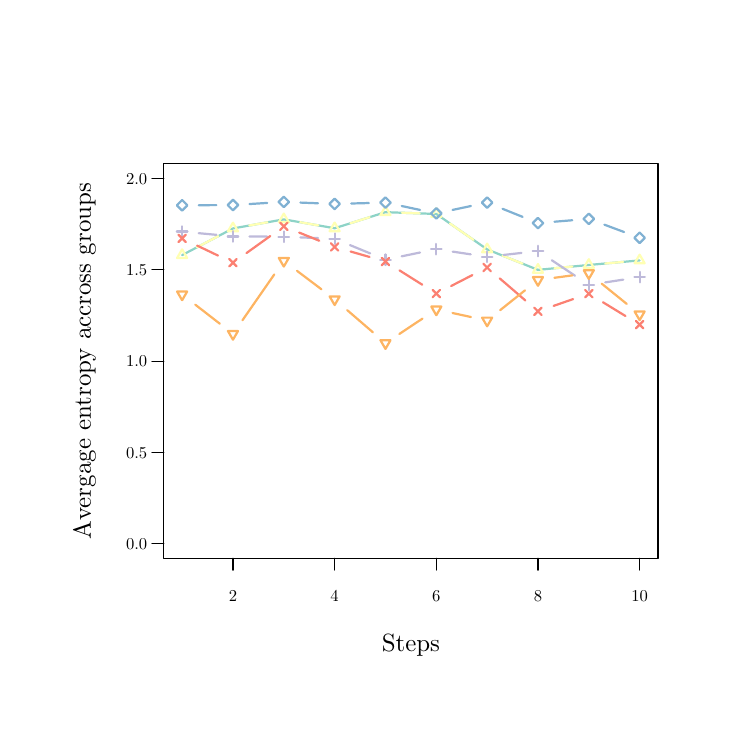
\begin{tikzpicture}[x=1pt,y=1pt]
\definecolor{fillColor}{RGB}{255,255,255}
\path[use as bounding box,fill=fillColor,fill opacity=0.00] (0,0) rectangle (252.94,252.94);
\begin{scope}
\path[clip] ( 49.20, 61.20) rectangle (227.75,203.75);
\definecolor{drawColor}{RGB}{141,211,199}

\path[draw=drawColor,line width= 0.8pt,line join=round,line cap=round] ( 55.81,170.76) --
	( 74.18,180.39) --
	( 92.55,183.67) --
	(110.92,180.46) --
	(129.29,186.27) --
	(147.66,185.62) --
	(166.03,172.82) --
	(184.39,165.42) --
	(202.76,167.19) --
	(221.13,168.84);
\end{scope}
\begin{scope}
\path[clip] (  0.00,  0.00) rectangle (252.94,252.94);
\definecolor{drawColor}{RGB}{0,0,0}

\path[draw=drawColor,line width= 0.4pt,line join=round,line cap=round] ( 74.18, 61.20) -- (221.13, 61.20);

\path[draw=drawColor,line width= 0.4pt,line join=round,line cap=round] ( 74.18, 61.20) -- ( 74.18, 56.92);

\path[draw=drawColor,line width= 0.4pt,line join=round,line cap=round] (110.92, 61.20) -- (110.92, 56.92);

\path[draw=drawColor,line width= 0.4pt,line join=round,line cap=round] (147.66, 61.20) -- (147.66, 56.92);

\path[draw=drawColor,line width= 0.4pt,line join=round,line cap=round] (184.39, 61.20) -- (184.39, 56.92);

\path[draw=drawColor,line width= 0.4pt,line join=round,line cap=round] (221.13, 61.20) -- (221.13, 56.92);

\node[text=drawColor,anchor=base,inner sep=0pt, outer sep=0pt, scale=  0.60] at ( 74.18, 45.60) {2};

\node[text=drawColor,anchor=base,inner sep=0pt, outer sep=0pt, scale=  0.60] at (110.92, 45.60) {4};

\node[text=drawColor,anchor=base,inner sep=0pt, outer sep=0pt, scale=  0.60] at (147.66, 45.60) {6};

\node[text=drawColor,anchor=base,inner sep=0pt, outer sep=0pt, scale=  0.60] at (184.39, 45.60) {8};

\node[text=drawColor,anchor=base,inner sep=0pt, outer sep=0pt, scale=  0.60] at (221.13, 45.60) {10};

\path[draw=drawColor,line width= 0.4pt,line join=round,line cap=round] ( 49.20, 66.48) -- ( 49.20,198.47);

\path[draw=drawColor,line width= 0.4pt,line join=round,line cap=round] ( 49.20, 66.48) -- ( 44.92, 66.48);

\path[draw=drawColor,line width= 0.4pt,line join=round,line cap=round] ( 49.20, 99.48) -- ( 44.92, 99.48);

\path[draw=drawColor,line width= 0.4pt,line join=round,line cap=round] ( 49.20,132.47) -- ( 44.92,132.47);

\path[draw=drawColor,line width= 0.4pt,line join=round,line cap=round] ( 49.20,165.47) -- ( 44.92,165.47);

\path[draw=drawColor,line width= 0.4pt,line join=round,line cap=round] ( 49.20,198.47) -- ( 44.92,198.47);

\node[text=drawColor,anchor=base east,inner sep=0pt, outer sep=0pt, scale=  0.60] at ( 43.20, 64.41) {0.0};

\node[text=drawColor,anchor=base east,inner sep=0pt, outer sep=0pt, scale=  0.60] at ( 43.20, 97.41) {0.5};

\node[text=drawColor,anchor=base east,inner sep=0pt, outer sep=0pt, scale=  0.60] at ( 43.20,130.41) {1.0};

\node[text=drawColor,anchor=base east,inner sep=0pt, outer sep=0pt, scale=  0.60] at ( 43.20,163.40) {1.5};

\node[text=drawColor,anchor=base east,inner sep=0pt, outer sep=0pt, scale=  0.60] at ( 43.20,196.40) {2.0};

\path[draw=drawColor,line width= 0.4pt,line join=round,line cap=round] ( 49.20, 61.20) --
	(227.75, 61.20) --
	(227.75,203.75) --
	( 49.20,203.75) --
	( 49.20, 61.20);
\end{scope}
\begin{scope}
\path[clip] (  0.00,  0.00) rectangle (252.94,252.94);
\definecolor{drawColor}{RGB}{0,0,0}

\node[text=drawColor,anchor=base,inner sep=0pt, outer sep=0pt, scale=  0.90] at (138.47, 27.60) {Steps};

\node[text=drawColor,rotate= 90.00,anchor=base,inner sep=0pt, outer sep=0pt, scale=  0.90] at ( 22.80,132.47) {Avergage entropy accross groups};
\end{scope}
\begin{scope}
\path[clip] ( 49.20, 61.20) rectangle (227.75,203.75);
\definecolor{drawColor}{RGB}{255,255,179}

\path[draw=drawColor,line width= 0.8pt,line join=round,line cap=round] ( 61.13,173.55) -- ( 68.87,177.61);

\path[draw=drawColor,line width= 0.8pt,line join=round,line cap=round] ( 80.09,181.45) -- ( 86.64,182.62);

\path[draw=drawColor,line width= 0.8pt,line join=round,line cap=round] ( 98.46,182.64) -- (105.01,181.49);

\path[draw=drawColor,line width= 0.8pt,line join=round,line cap=round] (116.64,182.27) -- (123.57,184.46);

\path[draw=drawColor,line width= 0.8pt,line join=round,line cap=round] (135.28,186.06) -- (141.66,185.83);

\path[draw=drawColor,line width= 0.8pt,line join=round,line cap=round] (152.58,182.19) -- (161.10,176.25);

\path[draw=drawColor,line width= 0.8pt,line join=round,line cap=round] (171.59,170.58) -- (178.83,167.66);

\path[draw=drawColor,line width= 0.8pt,line join=round,line cap=round] (190.37,166.00) -- (196.79,166.62);

\path[draw=drawColor,line width= 0.8pt,line join=round,line cap=round] (208.74,167.73) -- (215.16,168.30);

\path[draw=drawColor,line width= 0.8pt,line join=round,line cap=round] ( 55.81,172.86) --
	( 57.63,169.71) --
	( 53.99,169.71) --
	( 55.81,172.86);

\path[draw=drawColor,line width= 0.8pt,line join=round,line cap=round] ( 74.18,182.49) --
	( 76.00,179.34) --
	( 72.36,179.34) --
	( 74.18,182.49);

\path[draw=drawColor,line width= 0.8pt,line join=round,line cap=round] ( 92.55,185.77) --
	( 94.37,182.62) --
	( 90.73,182.62) --
	( 92.55,185.77);

\path[draw=drawColor,line width= 0.8pt,line join=round,line cap=round] (110.92,182.55) --
	(112.74,179.41) --
	(109.10,179.41) --
	(110.92,182.55);

\path[draw=drawColor,line width= 0.8pt,line join=round,line cap=round] (129.29,188.37) --
	(131.11,185.22) --
	(127.47,185.22) --
	(129.29,188.37);

\path[draw=drawColor,line width= 0.8pt,line join=round,line cap=round] (147.66,187.72) --
	(149.48,184.57) --
	(145.84,184.57) --
	(147.66,187.72);

\path[draw=drawColor,line width= 0.8pt,line join=round,line cap=round] (166.03,174.92) --
	(167.84,171.77) --
	(164.21,171.77) --
	(166.03,174.92);

\path[draw=drawColor,line width= 0.8pt,line join=round,line cap=round] (184.39,167.52) --
	(186.21,164.37) --
	(182.58,164.37) --
	(184.39,167.52);

\path[draw=drawColor,line width= 0.8pt,line join=round,line cap=round] (202.76,169.29) --
	(204.58,166.14) --
	(200.95,166.14) --
	(202.76,169.29);

\path[draw=drawColor,line width= 0.8pt,line join=round,line cap=round] (221.13,170.94) --
	(222.95,167.79) --
	(219.31,167.79) --
	(221.13,170.94);
\definecolor{drawColor}{RGB}{190,186,218}

\path[draw=drawColor,line width= 0.8pt,line join=round,line cap=round] ( 61.79,178.68) -- ( 68.21,178.08);

\path[draw=drawColor,line width= 0.8pt,line join=round,line cap=round] ( 80.18,177.48) -- ( 86.55,177.44);

\path[draw=drawColor,line width= 0.8pt,line join=round,line cap=round] ( 98.55,177.16) -- (104.92,176.90);

\path[draw=drawColor,line width= 0.8pt,line join=round,line cap=round] (116.47,174.37) -- (123.74,171.38);

\path[draw=drawColor,line width= 0.8pt,line join=round,line cap=round] (135.16,170.32) -- (141.78,171.69);

\path[draw=drawColor,line width= 0.8pt,line join=round,line cap=round] (153.59,172.01) -- (160.09,171.03);

\path[draw=drawColor,line width= 0.8pt,line join=round,line cap=round] (171.99,170.81) -- (178.43,171.54);

\path[draw=drawColor,line width= 0.8pt,line join=round,line cap=round] (189.39,168.89) -- (197.77,163.31);

\path[draw=drawColor,line width= 0.8pt,line join=round,line cap=round] (208.69,160.89) -- (215.20,161.89);

\path[draw=drawColor,line width= 0.8pt,line join=round,line cap=round] ( 53.90,179.25) -- ( 57.72,179.25);

\path[draw=drawColor,line width= 0.8pt,line join=round,line cap=round] ( 55.81,177.34) -- ( 55.81,181.16);

\path[draw=drawColor,line width= 0.8pt,line join=round,line cap=round] ( 72.27,177.51) -- ( 76.09,177.51);

\path[draw=drawColor,line width= 0.8pt,line join=round,line cap=round] ( 74.18,175.60) -- ( 74.18,179.42);

\path[draw=drawColor,line width= 0.8pt,line join=round,line cap=round] ( 90.64,177.40) -- ( 94.46,177.40);

\path[draw=drawColor,line width= 0.8pt,line join=round,line cap=round] ( 92.55,175.49) -- ( 92.55,179.31);

\path[draw=drawColor,line width= 0.8pt,line join=round,line cap=round] (109.01,176.65) -- (112.83,176.65);

\path[draw=drawColor,line width= 0.8pt,line join=round,line cap=round] (110.92,174.74) -- (110.92,178.56);

\path[draw=drawColor,line width= 0.8pt,line join=round,line cap=round] (127.38,169.10) -- (131.20,169.10);

\path[draw=drawColor,line width= 0.8pt,line join=round,line cap=round] (129.29,167.19) -- (129.29,171.01);

\path[draw=drawColor,line width= 0.8pt,line join=round,line cap=round] (145.75,172.91) -- (149.57,172.91);

\path[draw=drawColor,line width= 0.8pt,line join=round,line cap=round] (147.66,171.00) -- (147.66,174.82);

\path[draw=drawColor,line width= 0.8pt,line join=round,line cap=round] (164.12,170.13) -- (167.93,170.13);

\path[draw=drawColor,line width= 0.8pt,line join=round,line cap=round] (166.03,168.22) -- (166.03,172.04);

\path[draw=drawColor,line width= 0.8pt,line join=round,line cap=round] (182.49,172.22) -- (186.30,172.22);

\path[draw=drawColor,line width= 0.8pt,line join=round,line cap=round] (184.39,170.31) -- (184.39,174.12);

\path[draw=drawColor,line width= 0.8pt,line join=round,line cap=round] (200.85,159.98) -- (204.67,159.98);

\path[draw=drawColor,line width= 0.8pt,line join=round,line cap=round] (202.76,158.07) -- (202.76,161.89);

\path[draw=drawColor,line width= 0.8pt,line join=round,line cap=round] (219.22,162.80) -- (223.04,162.80);

\path[draw=drawColor,line width= 0.8pt,line join=round,line cap=round] (221.13,160.89) -- (221.13,164.71);
\definecolor{drawColor}{RGB}{251,128,114}

\path[draw=drawColor,line width= 0.8pt,line join=round,line cap=round] ( 61.23,174.20) -- ( 68.77,170.59);

\path[draw=drawColor,line width= 0.8pt,line join=round,line cap=round] ( 79.06,171.49) -- ( 87.67,177.65);

\path[draw=drawColor,line width= 0.8pt,line join=round,line cap=round] ( 98.11,178.89) -- (105.36,175.95);

\path[draw=drawColor,line width= 0.8pt,line join=round,line cap=round] (116.69,172.05) -- (123.52,170.09);

\path[draw=drawColor,line width= 0.8pt,line join=round,line cap=round] (134.36,165.23) -- (142.58,160.06);

\path[draw=drawColor,line width= 0.8pt,line join=round,line cap=round] (153.00,159.59) -- (160.69,163.53);

\path[draw=drawColor,line width= 0.8pt,line join=round,line cap=round] (170.57,162.35) -- (179.85,154.36);

\path[draw=drawColor,line width= 0.8pt,line join=round,line cap=round] (190.06,152.41) -- (197.10,154.86);

\path[draw=drawColor,line width= 0.8pt,line join=round,line cap=round] (207.89,153.71) -- (216.01,148.75);

\path[draw=drawColor,line width= 0.8pt,line join=round,line cap=round] ( 54.46,175.43) -- ( 57.16,178.13);

\path[draw=drawColor,line width= 0.8pt,line join=round,line cap=round] ( 54.46,178.13) -- ( 57.16,175.43);

\path[draw=drawColor,line width= 0.8pt,line join=round,line cap=round] ( 72.83,166.65) -- ( 75.53,169.35);

\path[draw=drawColor,line width= 0.8pt,line join=round,line cap=round] ( 72.83,169.35) -- ( 75.53,166.65);

\path[draw=drawColor,line width= 0.8pt,line join=round,line cap=round] ( 91.20,179.79) -- ( 93.90,182.49);

\path[draw=drawColor,line width= 0.8pt,line join=round,line cap=round] ( 91.20,182.49) -- ( 93.90,179.79);

\path[draw=drawColor,line width= 0.8pt,line join=round,line cap=round] (109.57,172.35) -- (112.27,175.05);

\path[draw=drawColor,line width= 0.8pt,line join=round,line cap=round] (109.57,175.05) -- (112.27,172.35);

\path[draw=drawColor,line width= 0.8pt,line join=round,line cap=round] (127.94,167.08) -- (130.64,169.78);

\path[draw=drawColor,line width= 0.8pt,line join=round,line cap=round] (127.94,169.78) -- (130.64,167.08);

\path[draw=drawColor,line width= 0.8pt,line join=round,line cap=round] (146.31,155.51) -- (149.01,158.21);

\path[draw=drawColor,line width= 0.8pt,line join=round,line cap=round] (146.31,158.21) -- (149.01,155.51);

\path[draw=drawColor,line width= 0.8pt,line join=round,line cap=round] (164.68,164.92) -- (167.38,167.62);

\path[draw=drawColor,line width= 0.8pt,line join=round,line cap=round] (164.68,167.62) -- (167.38,164.92);

\path[draw=drawColor,line width= 0.8pt,line join=round,line cap=round] (183.04,149.09) -- (185.74,151.79);

\path[draw=drawColor,line width= 0.8pt,line join=round,line cap=round] (183.04,151.79) -- (185.74,149.09);

\path[draw=drawColor,line width= 0.8pt,line join=round,line cap=round] (201.41,155.48) -- (204.11,158.18);

\path[draw=drawColor,line width= 0.8pt,line join=round,line cap=round] (201.41,158.18) -- (204.11,155.48);

\path[draw=drawColor,line width= 0.8pt,line join=round,line cap=round] (219.78,144.28) -- (222.48,146.98);

\path[draw=drawColor,line width= 0.8pt,line join=round,line cap=round] (219.78,146.98) -- (222.48,144.28);
\definecolor{drawColor}{RGB}{128,177,211}

\path[draw=drawColor,line width= 0.8pt,line join=round,line cap=round] ( 61.81,188.79) -- ( 68.18,188.82);

\path[draw=drawColor,line width= 0.8pt,line join=round,line cap=round] ( 80.17,189.21) -- ( 86.56,189.61);

\path[draw=drawColor,line width= 0.8pt,line join=round,line cap=round] ( 98.55,189.73) -- (104.92,189.48);

\path[draw=drawColor,line width= 0.8pt,line join=round,line cap=round] (116.92,189.40) -- (123.29,189.57);

\path[draw=drawColor,line width= 0.8pt,line join=round,line cap=round] (135.16,188.49) -- (141.79,187.08);

\path[draw=drawColor,line width= 0.8pt,line join=round,line cap=round] (153.53,187.08) -- (160.16,188.49);

\path[draw=drawColor,line width= 0.8pt,line join=round,line cap=round] (171.59,187.49) -- (178.83,184.57);

\path[draw=drawColor,line width= 0.8pt,line join=round,line cap=round] (190.37,182.82) -- (196.78,183.35);

\path[draw=drawColor,line width= 0.8pt,line join=round,line cap=round] (208.39,181.75) -- (215.51,179.10);

\path[draw=drawColor,line width= 0.8pt,line join=round,line cap=round] ( 53.90,188.76) --
	( 55.81,190.66) --
	( 57.72,188.76) --
	( 55.81,186.85) --
	( 53.90,188.76);

\path[draw=drawColor,line width= 0.8pt,line join=round,line cap=round] ( 72.27,188.85) --
	( 74.18,190.76) --
	( 76.09,188.85) --
	( 74.18,186.94) --
	( 72.27,188.85);

\path[draw=drawColor,line width= 0.8pt,line join=round,line cap=round] ( 90.64,189.97) --
	( 92.55,191.88) --
	( 94.46,189.97) --
	( 92.55,188.07) --
	( 90.64,189.97);

\path[draw=drawColor,line width= 0.8pt,line join=round,line cap=round] (109.01,189.24) --
	(110.92,191.15) --
	(112.83,189.24) --
	(110.92,187.33) --
	(109.01,189.24);

\path[draw=drawColor,line width= 0.8pt,line join=round,line cap=round] (127.38,189.73) --
	(129.29,191.64) --
	(131.20,189.73) --
	(129.29,187.83) --
	(127.38,189.73);

\path[draw=drawColor,line width= 0.8pt,line join=round,line cap=round] (145.75,185.83) --
	(147.66,187.74) --
	(149.57,185.83) --
	(147.66,183.92) --
	(145.75,185.83);

\path[draw=drawColor,line width= 0.8pt,line join=round,line cap=round] (164.12,189.73) --
	(166.03,191.64) --
	(167.93,189.73) --
	(166.03,187.83) --
	(164.12,189.73);

\path[draw=drawColor,line width= 0.8pt,line join=round,line cap=round] (182.49,182.33) --
	(184.39,184.24) --
	(186.30,182.33) --
	(184.39,180.42) --
	(182.49,182.33);

\path[draw=drawColor,line width= 0.8pt,line join=round,line cap=round] (200.85,183.85) --
	(202.76,185.76) --
	(204.67,183.85) --
	(202.76,181.94) --
	(200.85,183.85);

\path[draw=drawColor,line width= 0.8pt,line join=round,line cap=round] (219.22,177.01) --
	(221.13,178.92) --
	(223.04,177.01) --
	(221.13,175.10) --
	(219.22,177.01);
\definecolor{drawColor}{RGB}{253,180,98}

\path[draw=drawColor,line width= 0.8pt,line join=round,line cap=round] ( 60.55,152.86) -- ( 69.44,145.96);

\path[draw=drawColor,line width= 0.8pt,line join=round,line cap=round] ( 77.61,147.21) -- ( 89.12,163.77);

\path[draw=drawColor,line width= 0.8pt,line join=round,line cap=round] ( 97.33,165.07) -- (106.14,158.41);

\path[draw=drawColor,line width= 0.8pt,line join=round,line cap=round] (115.46,150.87) -- (124.74,142.87);

\path[draw=drawColor,line width= 0.8pt,line join=round,line cap=round] (134.29,142.26) -- (142.65,147.80);

\path[draw=drawColor,line width= 0.8pt,line join=round,line cap=round] (153.52,149.83) -- (160.16,148.39);

\path[draw=drawColor,line width= 0.8pt,line join=round,line cap=round] (170.72,150.85) -- (179.70,158.02);

\path[draw=drawColor,line width= 0.8pt,line join=round,line cap=round] (190.34,162.56) -- (196.82,163.43);

\path[draw=drawColor,line width= 0.8pt,line join=round,line cap=round] (207.42,160.45) -- (216.47,153.12);

\path[draw=drawColor,line width= 0.8pt,line join=round,line cap=round] ( 55.81,154.44) --
	( 57.63,157.59) --
	( 53.99,157.59) --
	( 55.81,154.44);

\path[draw=drawColor,line width= 0.8pt,line join=round,line cap=round] ( 74.18,140.18) --
	( 76.00,143.33) --
	( 72.36,143.33) --
	( 74.18,140.18);

\path[draw=drawColor,line width= 0.8pt,line join=round,line cap=round] ( 92.55,166.60) --
	( 94.37,169.74) --
	( 90.73,169.74) --
	( 92.55,166.60);

\path[draw=drawColor,line width= 0.8pt,line join=round,line cap=round] (110.92,152.69) --
	(112.74,155.83) --
	(109.10,155.83) --
	(110.92,152.69);

\path[draw=drawColor,line width= 0.8pt,line join=round,line cap=round] (129.29,136.85) --
	(131.11,140.00) --
	(127.47,140.00) --
	(129.29,136.85);

\path[draw=drawColor,line width= 0.8pt,line join=round,line cap=round] (147.66,149.01) --
	(149.48,152.16) --
	(145.84,152.16) --
	(147.66,149.01);

\path[draw=drawColor,line width= 0.8pt,line join=round,line cap=round] (166.03,145.01) --
	(167.84,148.16) --
	(164.21,148.16) --
	(166.03,145.01);

\path[draw=drawColor,line width= 0.8pt,line join=round,line cap=round] (184.39,159.66) --
	(186.21,162.81) --
	(182.58,162.81) --
	(184.39,159.66);

\path[draw=drawColor,line width= 0.8pt,line join=round,line cap=round] (202.76,162.13) --
	(204.58,165.28) --
	(200.95,165.28) --
	(202.76,162.13);

\path[draw=drawColor,line width= 0.8pt,line join=round,line cap=round] (221.13,147.24) --
	(222.95,150.39) --
	(219.31,150.39) --
	(221.13,147.24);
\end{scope}
\end{tikzpicture}
 & % Created by tikzDevice version 0.10.1 on 2016-06-15 20:08:04
% !TEX encoding = UTF-8 Unicode
\begin{tikzpicture}[x=1pt,y=1pt]
\definecolor{fillColor}{RGB}{255,255,255}
\path[use as bounding box,fill=fillColor,fill opacity=0.00] (0,0) rectangle (252.94,252.94);
\begin{scope}
\path[clip] ( 49.20, 61.20) rectangle (227.75,203.75);
\definecolor{drawColor}{RGB}{255,0,0}

\path[draw=drawColor,line width= 0.6pt,line join=round,line cap=round] ( 55.81, 66.48) --
	( 57.48,105.66) --
	( 59.15,130.95) --
	( 60.82,146.68) --
	( 62.49,156.23) --
	( 64.16,162.42) --
	( 65.83,166.50) --
	( 67.50,171.46) --
	( 69.17,175.06) --
	( 70.84,175.81) --
	( 72.51,177.66) --
	( 74.18,178.80) --
	( 75.85,179.50) --
	( 77.52,180.43) --
	( 79.19,180.93) --
	( 80.86,181.20) --
	( 82.53,181.82) --
	( 84.20,182.44) --
	( 85.87,183.08) --
	( 87.54,183.43) --
	( 89.21,184.38) --
	( 90.88,185.41) --
	( 92.55,185.93) --
	( 94.22,186.65) --
	( 95.89,187.17) --
	( 97.56,187.79) --
	( 99.23,188.41) --
	(100.90,188.61) --
	(102.57,188.65) --
	(104.24,188.92) --
	(105.91,189.20) --
	(107.58,189.35) --
	(109.25,189.62) --
	(110.92,189.69) --
	(112.59,189.86) --
	(114.26,189.90) --
	(115.93,189.97) --
	(117.60,190.08) --
	(119.27,190.23) --
	(120.94,190.13) --
	(122.61,190.21) --
	(124.28,190.18) --
	(125.95,190.13) --
	(127.62,190.08) --
	(129.29,190.07) --
	(130.96,190.14) --
	(132.63,190.16) --
	(134.30,190.10) --
	(135.97,190.13) --
	(137.64,190.09) --
	(139.31,190.06) --
	(140.98,190.16) --
	(142.65,190.16) --
	(144.32,190.09) --
	(145.99,190.18) --
	(147.66,190.18) --
	(149.33,190.18) --
	(151.00,190.21) --
	(152.67,190.27) --
	(154.34,190.29) --
	(156.01,190.36) --
	(157.68,190.40) --
	(159.35,190.43) --
	(161.02,190.41) --
	(162.69,190.49) --
	(164.36,190.52) --
	(166.03,190.51) --
	(167.70,190.54) --
	(169.37,190.50) --
	(171.04,190.49) --
	(172.71,190.51) --
	(174.38,190.56) --
	(176.05,190.53) --
	(177.71,190.56) --
	(179.38,190.58) --
	(181.05,190.53) --
	(182.72,190.47) --
	(184.39,190.44) --
	(186.06,190.45) --
	(187.73,190.39) --
	(189.40,190.41) --
	(191.07,190.42) --
	(192.74,190.40) --
	(194.41,190.41) --
	(196.08,190.37) --
	(197.75,190.39) --
	(199.42,190.33) --
	(201.09,190.32) --
	(202.76,190.29) --
	(204.43,190.27) --
	(206.10,190.32) --
	(207.77,190.30) --
	(209.44,190.23) --
	(211.11,190.30) --
	(212.78,190.31) --
	(214.45,190.31) --
	(216.12,190.26) --
	(217.79,190.25) --
	(219.46,190.29) --
	(221.13,190.22);
\end{scope}
\begin{scope}
\path[clip] (  0.00,  0.00) rectangle (252.94,252.94);
\definecolor{drawColor}{RGB}{0,0,0}

\path[draw=drawColor,line width= 0.4pt,line join=round,line cap=round] ( 54.14, 61.20) -- (221.13, 61.20);

\path[draw=drawColor,line width= 0.4pt,line join=round,line cap=round] ( 54.14, 61.20) -- ( 54.14, 56.92);

\path[draw=drawColor,line width= 0.4pt,line join=round,line cap=round] ( 87.54, 61.20) -- ( 87.54, 56.92);

\path[draw=drawColor,line width= 0.4pt,line join=round,line cap=round] (120.94, 61.20) -- (120.94, 56.92);

\path[draw=drawColor,line width= 0.4pt,line join=round,line cap=round] (154.34, 61.20) -- (154.34, 56.92);

\path[draw=drawColor,line width= 0.4pt,line join=round,line cap=round] (187.73, 61.20) -- (187.73, 56.92);

\path[draw=drawColor,line width= 0.4pt,line join=round,line cap=round] (221.13, 61.20) -- (221.13, 56.92);

\node[text=drawColor,anchor=base,inner sep=0pt, outer sep=0pt, scale=  0.50] at ( 54.14, 45.60) {0};

\node[text=drawColor,anchor=base,inner sep=0pt, outer sep=0pt, scale=  0.50] at ( 87.54, 45.60) {20};

\node[text=drawColor,anchor=base,inner sep=0pt, outer sep=0pt, scale=  0.50] at (120.94, 45.60) {40};

\node[text=drawColor,anchor=base,inner sep=0pt, outer sep=0pt, scale=  0.50] at (154.34, 45.60) {60};

\node[text=drawColor,anchor=base,inner sep=0pt, outer sep=0pt, scale=  0.50] at (187.73, 45.60) {80};

\node[text=drawColor,anchor=base,inner sep=0pt, outer sep=0pt, scale=  0.50] at (221.13, 45.60) {100};

\path[draw=drawColor,line width= 0.4pt,line join=round,line cap=round] ( 49.20, 66.48) -- ( 49.20,198.47);

\path[draw=drawColor,line width= 0.4pt,line join=round,line cap=round] ( 49.20, 66.48) -- ( 44.92, 66.48);

\path[draw=drawColor,line width= 0.4pt,line join=round,line cap=round] ( 49.20, 99.48) -- ( 44.92, 99.48);

\path[draw=drawColor,line width= 0.4pt,line join=round,line cap=round] ( 49.20,132.47) -- ( 44.92,132.47);

\path[draw=drawColor,line width= 0.4pt,line join=round,line cap=round] ( 49.20,165.47) -- ( 44.92,165.47);

\path[draw=drawColor,line width= 0.4pt,line join=round,line cap=round] ( 49.20,198.47) -- ( 44.92,198.47);

\node[text=drawColor,anchor=base east,inner sep=0pt, outer sep=0pt, scale=  0.50] at ( 43.20, 64.76) {0.0};

\node[text=drawColor,anchor=base east,inner sep=0pt, outer sep=0pt, scale=  0.50] at ( 43.20, 97.75) {0.5};

\node[text=drawColor,anchor=base east,inner sep=0pt, outer sep=0pt, scale=  0.50] at ( 43.20,130.75) {1.0};

\node[text=drawColor,anchor=base east,inner sep=0pt, outer sep=0pt, scale=  0.50] at ( 43.20,163.75) {1.5};

\node[text=drawColor,anchor=base east,inner sep=0pt, outer sep=0pt, scale=  0.50] at ( 43.20,196.74) {2.0};

\path[draw=drawColor,line width= 0.4pt,line join=round,line cap=round] ( 49.20, 61.20) --
	(227.75, 61.20) --
	(227.75,203.75) --
	( 49.20,203.75) --
	( 49.20, 61.20);
\end{scope}
\begin{scope}
\path[clip] (  0.00,  0.00) rectangle (252.94,252.94);
\definecolor{drawColor}{RGB}{0,0,0}

\node[text=drawColor,anchor=base,inner sep=0pt, outer sep=0pt, scale=  0.80] at (138.47, 27.60) {Steps};

\node[text=drawColor,rotate= 90.00,anchor=base,inner sep=0pt, outer sep=0pt, scale=  0.80] at ( 22.80,132.47) {Avergage entropy};
\end{scope}
\begin{scope}
\path[clip] ( 49.20, 61.20) rectangle (227.75,203.75);
\definecolor{drawColor}{RGB}{0,0,255}

\path[draw=drawColor,line width= 0.4pt,line join=round,line cap=round] ( 55.81, 66.48) --
	( 57.48,111.70) --
	( 59.15,138.88) --
	( 60.82,156.80) --
	( 62.49,164.40) --
	( 64.16,167.85) --
	( 65.83,168.98) --
	( 67.50,171.17) --
	( 69.17,172.29) --
	( 70.84,173.25) --
	( 72.51,174.80) --
	( 74.18,175.50) --
	( 75.85,176.38) --
	( 77.52,176.77) --
	( 79.19,177.07) --
	( 80.86,177.64) --
	( 82.53,177.72) --
	( 84.20,178.30) --
	( 85.87,178.45) --
	( 87.54,178.47) --
	( 89.21,178.64) --
	( 90.88,178.83) --
	( 92.55,178.78) --
	( 94.22,179.06) --
	( 95.89,179.14) --
	( 97.56,179.47) --
	( 99.23,179.59) --
	(100.90,179.94) --
	(102.57,180.10) --
	(104.24,180.14) --
	(105.91,180.36) --
	(107.58,180.51) --
	(109.25,180.68) --
	(110.92,180.88) --
	(112.59,181.01) --
	(114.26,181.25) --
	(115.93,181.40) --
	(117.60,181.40) --
	(119.27,181.43) --
	(120.94,181.49) --
	(122.61,181.62) --
	(124.28,181.69) --
	(125.95,181.75) --
	(127.62,181.87) --
	(129.29,181.85) --
	(130.96,181.78) --
	(132.63,181.78) --
	(134.30,181.85) --
	(135.97,181.74) --
	(137.64,181.79) --
	(139.31,181.77) --
	(140.98,181.86) --
	(142.65,181.90) --
	(144.32,181.88) --
	(145.99,181.84) --
	(147.66,181.78) --
	(149.33,181.85) --
	(151.00,181.85) --
	(152.67,181.91) --
	(154.34,181.95) --
	(156.01,181.96) --
	(157.68,181.85) --
	(159.35,181.80) --
	(161.02,181.84) --
	(162.69,181.79) --
	(164.36,181.78) --
	(166.03,181.71) --
	(167.70,181.61) --
	(169.37,181.60) --
	(171.04,181.64) --
	(172.71,181.60) --
	(174.38,181.59) --
	(176.05,181.59) --
	(177.71,181.60) --
	(179.38,181.56) --
	(181.05,181.58) --
	(182.72,181.55) --
	(184.39,181.49) --
	(186.06,181.45) --
	(187.73,181.42) --
	(189.40,181.40) --
	(191.07,181.29) --
	(192.74,181.20) --
	(194.41,181.08) --
	(196.08,181.06) --
	(197.75,181.04) --
	(199.42,180.98) --
	(201.09,180.97) --
	(202.76,180.94) --
	(204.43,180.93) --
	(206.10,180.91) --
	(207.77,180.88) --
	(209.44,180.84) --
	(211.11,180.79) --
	(212.78,180.79) --
	(214.45,180.76) --
	(216.12,180.64) --
	(217.79,180.54) --
	(219.46,180.45) --
	(221.13,180.36);
\definecolor{drawColor}{RGB}{255,0,0}

\path[draw=drawColor,line width= 0.4pt,line join=round,line cap=round] (198.23, 78.00) -- (205.43, 78.00);
\definecolor{drawColor}{RGB}{0,0,255}

\path[draw=drawColor,line width= 0.4pt,line join=round,line cap=round] (198.23, 68.40) -- (205.43, 68.40);
\definecolor{drawColor}{RGB}{0,0,0}

\node[text=drawColor,anchor=base west,inner sep=0pt, outer sep=0pt, scale=  0.40] at (209.03, 76.62) {Criminals};

\node[text=drawColor,anchor=base west,inner sep=0pt, outer sep=0pt, scale=  0.40] at (209.03, 67.02) {Controll};
\end{scope}
\end{tikzpicture}
 \\
	(c) Average Entropy across groups & (d) Blockwise picks from disadvantageous deck 
	\end{tabular}
	\caption{Average py and disadvantageous behaviour}
	\label{fig:ent}
\end{figure}

Yechiam et al. found three clusters by using the attention to recent outcomes(ARO) and attention to gains(AG) parameters from the Expectancy Valance model. The most distinct group were the Robbery convicts with the only negative attention to gains mean at -0.36 and the highest attention to recent outcomes mean 0.57. The second cluster is made of assault and murder convicts with ARO of 0.26 and AG of 0.1. The third cluster is formed of all the remaining prisoner groups with ARO means between 0 and -0.1 and AG between 0.1 and 0.2.
Based on those findings and what we observed in figure \ref{fig:ent} we decided to cluster convicted assault-murder and robbery individuals against the other criminal groups. The following table depicts the resulting clustering performance.

\subsection{Huntington Data}

\cite{Stout2001} conducted research on behaviour of patients with Huntington disease (HD) and Parkinson disease (PD).\footnote{The Huntington Disease is an illness of the central nervous system. The are are a wide range of associated symptoms including physical symptoms like uncontrollable muscular movements and clumsiness and psychological symptoms like minored concentration, short term memory lapses etc . Moreover a related possible symptom is Parkinson disease \cite{hunt}. Parkinson is chronic and progressive movement  disorder. Also Parkinson goes along with physical, such as tremors and rigidity and psychological symptoms, such as memory problems, minored speed of thinking fear and anxiety (among others) \cite{parc}} 
In the study there were considered 14 participants with HD and 22 participants with PD. They participants are required to don't have ongoing drug problems (including alcohol), free of other major diseases (physical or psychological nature). A group of 33 people serves as a control group. This group can further distinguished in younger (YHC) and older control participants (OHC). Table \ref{tab:hus} gives a basic summary of the demographic of the participants.

\setlength{\tabcolsep}{10pt}
\renewcommand{\arraystretch}{1}
\begin{table}[H]
	\centering 
	\scriptsize
	\begin{tabularx}{\textwidth}{lccccc}
		\toprule
		\textbf{Demographic} & \textbf{Hunting Disease} & \textbf{Parkinson Disease} & \textbf{YHC} & \textbf{OHF} \\
		\hline
		Age & 		44.60 (11.70) & 66.00 (8.30) & 45.30 (10.60) & 65.50 (10.70) \\
		Education (years) & 15.30 (2.30) & 14.20 (2.90) & 14.30 (2.10) &14.70 (2.40) \\
		Sex & 130.60 (10.10) & 131.70 (7.60) & 139.50 (2.20) & 138.00 (4.60) \\
		Years since diagnosis & 4.10 (2.80) & 7.70 (5.50) & NA (NA) & NA (NA) \\
		Estimated age at diagnosis & 40.50 (10.80) & 58.30 (7.60) & NA (NA) & NA (NA) \\
		\bottomrule
	\end{tabularx}
	\caption{Shortened summary of HD, PD and control people (means with standard deviations in parenthesis)}
	\label{tab:hus}
	\textbf{Source:} Summary of \cite[page 3]{Stout2001} 
\end{table}

\subsection{Cocaine Abusers data}

Finally we study data from several cocaine abusers. There are 12 individuals performing the IGT. The control group consist out of 14 participants. Candidates among the drug abusers were selected as active users with additional drug abusing past, but without any known additional mental illness \cite{stout2004}. Table \ref{tab:cocs} gives a summary of demographic profile.

\setlength{\tabcolsep}{12pt}
\renewcommand{\arraystretch}{1}
\begin{table}[H]
	\centering 
	\begin{tabular}{lcc}
		\toprule
		\textbf{demographic} & \textbf{Drug abusers} & \textbf{Control Group} \\
		\hline
		Share of men &  79\% & 100\%\\
		Age & 36.90 (10.30) & 30.00 (6.10) \\
		Estimated IQ & 105.00 (7.62) & 93.70 (10.30) \\
		\bottomrule
	\end{tabular}
	\caption{Demographic summary of cocaine abusers (means with standard deviations in parenthesis)}
	\label{tab:cocs}
\end{table}

We cluster cocaine abusers against the control group. The following table depicts results of the clustering. Again we averaged over 20 simulations to report average clustering performance. However as depicted the data set is friarly small and results are quite stable. Again our best clustering is achieved using block wise entropy, besides the listed K-Means algorithm, spectral clustering with both cosine similarity and with and rbf kernel achieved the same results. However, the results for this data set are in general are rather low and a real good clustering performance can not be found indicated by the average over all applied methods. 

\begin{threeparttable}[H] 
	\centering
	\label{} 
	\scriptsize
		\resizebox{\textwidth}{!}{\begin{tabular}{ llccc cccccc} 
		\toprule
		Method & Similarity & C\tnote{0} & CBC\tnote{1} & BBC\tnote{2} & E\tnote{3} & EB\tnote{4} & CC\tnote{5} & NMI\tnote{6} & ARI\tnote{6} & VM\tnote{7} \\ 
		\hline 
		K-Means \tnote{*} & Euclidian &  &  &  &  & x &  & 0.270 (0.000) & 0.262 (0.000) & 0.270 (0.000) \\ 
		Ward & Euclidian &  & x &  &  &  &  & 0.270 (0.000) & 0.262 (0.000) & 0.270 (0.000) \\ 
		K-Means & Euclidian &  &  &  &  &  & x & 0.209 (0.030) & 0.171 (0.043) & 0.208 (0.030) \\ 
		Spectral & Levenstein & x &  &  &  &  &  & 0.178 (0.000) & 0.181 (0.000) & 0.178 (0.000) \\ 
		Spectral & Cosine &  &  & x &  &  &  & 0.171 (0.000) & 0.117 (0.000) & 0.171 (0.000) \\ 
		Spectral & DTW &  &  &  & x &  &  & 0.042 (0,000) & 0.014 (0.000) & 0.042 (0.000) \\ 
		\hline
		\textbf{Average}\tnote{$\dagger$}  & - & - & - & - & - & - & - & 0.139 (0.002) & 0.104 (0.003) & 0.138 (0.002) \\ 
		\hline 
	\end{tabular} }
	\begin{tcolorbox}[arc=0mm,title=Notes,boxrule=0.2mm,colbacktitle=white,coltitle=black,colback=white,top=0mm,bottom=0.1mm]
	\begin{tablenotes}
	       	\item[0] Clustering based on choices participant did 
	       	\item[1] Clustering based on cumulative disadvantageous choice of participants
	        \item[2] Clustering based on block wise disadvantageous choice. Block size = 10
	        \item[3] Clustering based on cumulative entropy
	        \item[4] Clustering based on block wise entropy. Block size = 10
	        \item[5] Clustering based on entropy and choices concatenated for each participant
	        \item[6] Normalised mutual infrormation score (description see appendix \ref{sec:ce})
	        \item[7] Adjusted rand index (description see appendix \ref{sec:ce})
	        \item[8] V-Measure (description see appendix \ref{sec:ce})
	        \item[*] Spectral Clustering on block wise entropy with RBF kernel and cosine similarity produced the same results
	        \item[$\dagger$] Average over all algorithms including the ones displayed in the table
	\end{tablenotes}
	\end{tcolorbox}
	\caption{Clustering results for cocaine abusers vs. control group} 
 \end{threeparttable} 

\section{Discussion of results and possible extensions }

Our analysis so far showed that people are not separate themselves. In general we assume that healthy participants and those with assumed decision making deficits show significantly different behaviour. However, we observe that their behaviour seem to be quite similar given our data and applied mappings. Furthermore , in most of the applied unsupervised techniques we as analysts have to to set the number of clusters we assume to be in the data (so in our case two for control group and patients with habits). We apply another algorithm called affinity propagation, which identifies the number of clusters itself (algorithm formulation see appendix). In general we find that the algorithm is assign , which suggest that there more natural clusters in the data than the  one we assume due to their status labeled as healthy and ill.

%---------------------------------------------------------------------------------------------------------
% 5. Data
%---------------------------------------------------------------------------------------------------------

\section{Conclusion}


\section{Acknowledgment}




\pagebreak
% ----------------------------------------------------------------------------------------------------------
% Literature
% ----------------------------------------------------------------------------------------------------------

\renewcommand\refname{List of Literature}

\bibliographystyle{apalike}

\bibliography{unsupervised}


\pagebreak

%----------------------------------------------------------------------------------------------------------
% Appendix
% ---------------------------------------------------------------------------------------------------------
\lhead{Appendix \thesection}
\rhead{}
\pagenumbering{Alph}
\setcounter{page}{1}

\begin{appendix}
	
\section*{Appendix}
\phantomsection
\addcontentsline{toc}{section}{Appendix}
\addtocontents{toc}{\vspace{-0.5em}}

\subsection*{Metrics and Similarities}

This part of the appendix formally defines metrics and similarities and dissimilarities (proximity) used in this paper. We first define some basic general concepts followed by a description of the applied distance and similarity concepts. 

\subsubsection*{Distances vs. Similarities}

Let $\mathcal{X}$ be a dataset and let $\boldsymbol{x_i},\boldsymbol{x_j}$ be two datapoints, such that $\boldsymbol{x_i},\boldsymbol{x_j} \in \mathcal{X}$. 

A distance function assign for pairs a points a non negative real number as distance. $d:\mathcal{X}\times \mathcal{X} \mapsto \mathbb{R}_0^+$. Formally if the following properties are additionally staisfied the distance is also metric \cite[page 28]{Shirali06a}.

\begin{enumerate}
	\setlength{\itemsep}{-5pt}
	\item $d(\boldsymbol{x_i},\boldsymbol{x_j}) \ge 0$
	\item $d(\boldsymbol{x_i},\boldsymbol{x_i}) \ge 0$
	\item $d(\boldsymbol{x_i},\boldsymbol{x_j}) = d(\boldsymbol{x_j},\boldsymbol{x_i}) $
	\item $d(\boldsymbol{x_i},\boldsymbol{x_j}) \le d(\boldsymbol{x_i},\boldsymbol{x_j})+ d(\boldsymbol{x_j},\boldsymbol{x_i}) $
\end{enumerate}

A distance can be seen as a measure for dissimilarity of two points \cite[page 35]{Everitt2009}. Besides distance some algorithms operate on a \textit{similarity} matrix. Formally a similarity is a function  $ S : \mathcal{X} \times \mathcal{X} \mapsto [0,1] $. Also for similarity we can define the following properties \cite[page 3]{Fratev1979}:

\begin{enumerate}
	\setlength{\itemsep}{-5pt}
	\item $0 \le S(\boldsymbol{x_i},\boldsymbol{x_j}) \le 1, \text{for } i \neq j$
	\item $S(\boldsymbol{x_i},\boldsymbol{x_i}) = 1$
	\item $S(\boldsymbol{x_i},\boldsymbol{x_j}) = S(\boldsymbol{x_j},\boldsymbol{x_i})$
\end{enumerate}

Once we have computed distance or a similarity we can compute for two data points we can use this information to transform it to a similarity or the distance vice versa \cite[page 4]{Boriah2008}:

\begin{flalign}
S(\boldsymbol{x_i},\boldsymbol{x_j}) = \frac{1}{1+d(\boldsymbol{x_i},\boldsymbol{x_j}) } \hspace{0.5cm} \Leftrightarrow \hspace{0.5cm} d(\boldsymbol{x_i},\boldsymbol{x_j}) =  \frac{1}{S(\boldsymbol{x_i},\boldsymbol{x_j})} -1 
\label{eq:sim}
\end{flalign}

\subsubsection{Similarity measures for time series data}

We use three different similarity measures for time series. E.g. \cite{Wang2013} or \cite{Serr2014} provide an overview and empirical evaluation on common similarity measures for time series. The following definitions are taken from the latter. Empirical research suggest that simple euclidean distance for time series performs quite well and is hard to beat. Hence, the first distance measure for time series is simply euclidean distance between two time series. They might be converted to similarity based on equation \ref{eq:sim}. Let $\boldsymbol{x},\boldsymbol{y}$ be two time series over N-periods. Then the $L_2$ distance between two time series is define as: 

\begin{flalign}
d_E (\boldsymbol{x},\boldsymbol{y}) :=  \sqrt{\left( \sum_{i=1}^{N} \left( x_i - y_i \right)^2 \right)}
\label{eq:ets}
\end{flalign}
\pagebreak

\subsubsection{Similarity measures for categorical data}

Reffering to equation \ref{eq:ets} we define a simple measure for the categorical aspect of the data. Note that [SOURCE] defines the simplest measure for categorical data. However, since the probability that two people behave exactly the same in our context is arguably zero we modify this concept slightly. So we relax that and define the overlap similarity just as the count of overlapping instances. This serves as a benchmark similarity for categorical data.

\footnote{For example Levenstein distance (or edit distance) is a basic way to measure similarity between categorical sequences \cite[page 1]]{Richter} or \cite[page 2]{Gabadinho2009}, however some authors stating that it might perform poorly in their task \cite[page 3]{Ren2011} or a poor measure at all \cite[page 5]{Morzy}}


\begin{flalign}
d_O (\boldsymbol{x},\boldsymbol{y}) :=  \sum_{i=1}^{N} \mathbb{1}_{(x_i = y_i)}
\end{flalign}

In [Boriah 2008] we find a rich class of further categorical measures. To keep it concise we considered two of them. The first one is \textit{Eskin} similarity measures.

\begin{flalign}
d_O (\boldsymbol{x},\boldsymbol{y}) := \begin{cases} 
1 & \text{,if } \boldsymbol{x} = \boldsymbol{y}  \\
\frac{n_k^2} {n_k^2 + 2} & \text{otherwise }
\end{cases}
\label{eq:esk}
\end{flalign}

Furthermore, we consider lins similarity 

\begin{flalign}
d_{lin} (\boldsymbol{x},\boldsymbol{y}) := \begin{cases} 
2 \log \hat{p}_k (X_k) & \text{,if } \boldsymbol{x} = \boldsymbol{y}  \\
2 \log \left( \hat{p}_k (x_k) + \hat{p}_k (y_k)\right) & \text{otherwise }
\end{cases}
\label{eq:esk}
\end{flalign}




\subsection*{Clustering Evaluation}
\label{sec:ce}
In this section we formally derive and explain the applied clustering metrics. Evaluating clustering performance has some issues. The algorithm is producing labels. Nevertheless we generated the "true" labels the might not be comparable. A simple example we might consider the following situation. Let y denote the labels of data the data and $y'$ the corresponding prediction such that  $y,y' \in \{0,1\}$. In a small example let our data points be like $y=(1,1,0,0)$ and the corresponding prediction $y'=(0,0,1,1)$. Obviously the clustering worked perfectly, however comparing "labels" would produce an accuracy of zero. 

There a several clustering metrics, which respect such a situation. We consider a bunch of information based metrics. Most of the measures use some sort of entropy. The following concepts can be found in \cite{Rosenberg2007} and  \cite{Vinh2010} and as additional reading \cite{Hubert1985}. 

First we might introduce the contingency table. 

\setlength{\tabcolsep}{0.2cm}
\renewcommand{\arraystretch}{1}
\begin{table}[htb]
	\centering
	\begin{tabular}{c | c c c c| c}
		 & $V_1$ & $V_2$ & $\dots$ & $V_c$ & $\Sigma$ \\
		\hline
		$U_1$ & $n_{1,1}$ &$n_{1,2}$  &$\dots$ & & $a_1$ \\ 
		$U_2$ & $n_{2,1}$ & $\ddots$ & & & $a_1$ \\ 
		$\vdots$ & $n_{1,1}$ & $\dots$ & & & $a_1$ \\ 
		$U_R$ & $n_{1,1}$ & $\dots$ & & & $a_1$ \\ 
		\hline
		& $b_1$ & $b_2$ & $\dots$ & $b_c$ & N
	\end{tabular}
\caption{Contigency Table}
\end{table}


\begin{tabbing}
	\hspace*{1cm}\=\hspace*{1cm}\=\hspace*{3cm}\=\hspace*{2.7cm}\= \kill
	\onehalfspacing
	\textbf{$N_{11}$:} \>\> Number of pairs in the same cluster \\ 
	\textbf{$N_{00}$:} \>\> Number of pairs that are in different clusters in both $v$ and $u$ \\ 
	\textbf{$N_{01}$:} \>\> Number of pairs that are in the same cluster in both $u$ but different in $v$ \\ 
	\textbf{$N_{10}$:} \>\>  Number of pairs that are in the same cluster in both $v$ but different in $u$ \\ 
\end{tabbing}

\begin{flalign}
RI(u,v) = \frac{N_{00}+N_{11}}{\binom{N}{2}}
\label{eq:ri}
\end{flalign}

\begin{flalign}
ARI(u,v) = \frac{2 \left(N_{00}N_{11} - N_{01} N_{10} \right)}{\left(N_{00} + N_{01} \right)\left( N_{01} + N_{11}\right) + \left(N_{00} + N_{10} \right)\left( N_{10} + N_{11}\right)}
\label{eq:ri}
\end{flalign}

\begin{flalign}
H(u) &= - \sum_{i=1}^{R} \frac{a_i}{N} \log  \frac{a_i}{N} \\
H(v) &= - \sum_{i=1}^{C} \frac{b_i}{N} \log  \frac{a_i}{N} \\
H(u,v) &= - \sum_{i=1}^{R}  \sum_{j=1}^{C}  \frac{n_{i,j}}{N} \log \frac{n_{i,j}}{N} \\ 
H(u|v) &= - \sum_{i=1}^{R}  \sum_{j=1}^{C}  \frac{n_{i,j}}{N} \log \frac{n_{i,j}/N}{b_j/N} \\
H(v|u) &= - \sum_{i=1}^{C}  \sum_{j=1}^{R}  \frac{n_{i,j}}{N} \log \frac{n_{i,j}/N}{b_j/N} \\
I(u,v) &= \sum_{i=1}^{R}  \sum_{j=1}^{C}  \frac{n_{i,j}}{N} \log \frac{n_{i,j}/N}{a_i b_j/N} \\
\end{flalign}

Normalized Info Score:

This is one example of a normalized version 
\begin{flalign}
NMI_{max}(u,v) = \frac{I(u,v)}{\max\left( H(u),H(v)\right)}
\end{flalign}


\begin{flalign}
AMI_{max}(u,v) &= \frac{NMI_{max}(u,v) - \mathbb{E}\left[NMI_{max}(u,v)\right] }{1-\mathbb{E}\left[ NMI_{max}(u,v)\right]} \nonumber \\ 
&=\frac{I(u,v) - \mathbb{E}\left[ I(u,v)\right]}{ \max \left(H(u), H(v)\right) - \mathbb{E}\left[ I(u,v)\right] }
\end{flalign}

\begin{flalign}
\mathbb{E}\left[I(u,v) \right] = \sum_{i=1}^{R}  \sum_{j=1}^{C} \sum_{ n_{i,j}=\max \left(a_i + b_j-N,0\right) }^{ \min \left( a,b \right) } \frac{n_{ij}}{N} \log \left( \frac{N n_{ij}}{a_i b_j} \right) \frac{a_i! b_j!(N-a_i)!(N-b_j)!}{N! n_{ij}! (a_i-n_{ij})(b_j - n_{ij})!(N-a_i-b_j+n_{ij})!}
\end{flalign}

Homogeneity: 

\begin{flalign}
h = \begin{cases} 
1 & \text{,if } H(u,v) = 0 \\
1 - \frac{H(u|v)} {H(u)} & \text{otherwise}
\end{cases}
\end{flalign}

Completeness:
\begin{flalign}
c = \begin{cases} 
1 & \text{,if } H(v,u) = 0 \\
1 - \frac{H(v|u)} {H(v)} & \text{otherwise}
\end{cases}
\end{flalign}

V Measure Score:

\begin{flalign}
V_\beta = \frac{(1+\beta)h c}{\beta h + c}
\end{flalign}


\subsection{Algorithms}


\subsubsection*{Principal Components and Multidimensional Scaling}

Coming to principal component analysis. \cite{Shlens2014} provides an excellent contribution considering both practical applications and theoretical background. The following derivations are from this source. 

\pagebreak
\subsubsection*{Spectral Clustering}

For the spectral clustering algorithm we formally introduce some graph notation. If not stated otherwise the following derivation follows \cite{Luxburg2007}. In the following we consider a weighted and simple undirected graph. 
\begin{flalign}
G &= \{V,E\} \\
V & = \{ v_1,\dots,v_n \} \\
E & = \{e_1,\dots,e_n\} 
\intertext{Furthermore let the graph has a weighted and symetric ($|V| \times |V|$) adjacency matrix, such that:}
\boldsymbol{W} &= \begin{cases} 
w_{i,j} & \text{,if } v_iv_j \in E \\
0 & \text{otherwise }
\end{cases}
\intertext{The \textit{degree} of a node is defined as the sum of edge weights of connected nodes. Formmally we denote the degree of node $i$ as:}
d_i &:= \sum_{j=1}^{n} w_{ij} = \sum_{i=1}^{n} w_{ij}
\intertext{Using the last expression we define matrix $\boldsymbol{D}$ as the diagonal matrix of the degress}
\boldsymbol{D} &:= diag(\boldsymbol{d})
\intertext{The algorithm works on the \textit{Laplacian} matrix defined by:}
\boldsymbol{L} &:= \boldsymbol{D} - \boldsymbol{W} 
\intertext{Former versions of the algorithm are applied on the graph laplcian. However, there were proposed newer versions using the so called \textit{normalized laplacian}. Since also the python version is using this package we will focus on this version of the algorithm. Following that the normalized graph laplacian is defined as:}
\boldsymbol{L}_{norm} &:= \boldsymbol{D}^{1/2} \boldsymbol{L} \boldsymbol{D}^{1/2}  = \boldsymbol{I} - \boldsymbol{D}^{1/2} \boldsymbol{W} \boldsymbol{D}^{1/2}
\end{flalign}

\section{Affinity Propagation}

\cite{Brusco2008}

\pagebreak
\section{Simulation Data}

\begin{table}[H] \centering 
	\label{} 
	\scriptsize
	\begin{tabularx}{\textwidth}{ ccccccccccc} 
		\\\toprule
		Tau & Method & Similarity & C & BBC & E & EB & CC & NMI & ARI & VM \\ 
		\hline \\[-1.8ex] 
		\{0.1, 0.3\} & Spectral & DTW &  &  &  & x &  & 0.136 (0.134) & 0.094 (0.146) & 0.135 (0.134) \\ 
		& Spectral & EDR &  &  & x &  &  & 0.134 (0.135) & 0.097 (0.130) & 0.134 (0.135) \\ 
		& Spectral & Levensthein & x &  &  &  &  & 0.093 (0.134) & 0.050 (0.128) & 0.092 (0.134) \\ 
		& Spectral & Cosine &  & x &  &  &  & 0.113 (0.134) & 0.082 (0.150) & 0.113 (0.134) \\ 
		& K-Means & Euclidian &  &  &  &  & x & 0.093 (0.135) & 0.050 (0.130) & 0.092 (0.135) \\ 
		\{0.1, 0.5\} & Spectral & RBF &  &  &  & x &  & 0.331 (0.185) & 0.328 (0.208) & 0.331 (0.186) \\ 
		& Spectral & RBF &  &  & x &  &  & 0.322 (0.197) & 0.301 (0.221) & 0.321 (0.197) \\ 
		& Spectral & EDR &  &  & x &  &  & 0.315 (0.189) & 0.328 (0.206) & 0.315 (0.189) \\ 
		& K-Means & Euclidian &  &  & x &  &  & 0.313 (0.187) & 0.261 (0.213) & 0.312 (0.187) \\ 
		& Spectral & EDR &  & x &  &  &  & 0.226 (0.127) & 0.131 (0.113) & 0.223 (0.127) \\ 
		& Spectral & Levensthein & x &  &  &  &  & 0.219 (0.144) & 0.126 (0.121) & 0.217 (0.144) \\ 
		& K-Means & Euclidian &  &  &  &  & x & 0.208 (0.143) & 0.124 (0.122) & 0.207 (0.143) \\ 
		\{0.1, 0.7\} & Spectral & RBF &  &  &  & x &  & 0.642 (0.200) & 0.653 (0.206) & 0.641 (0.200) \\ 
		& Spectral & DTW &  &  & x &  &  & 0.580 (0.209) & 0.611 (0.205) & 0.580 (0.201) \\ 
		& K-Means & Euclidian &  &  & x &  &  & 0.533 (0.248) & 0.539 (0.275) & 0.533 (0.249) \\ 
		& K-Means & Euclidian &  &  &  &  & x & 0.382 (0.181) & 0.309 (0.237) & 0.381 (0.180) \\ 
		& Spectral & Levensthein & x &  &  &  &  & 0.350 (0.114) & 0.241 (0.163) & 0.347 (0.116) \\ 
		& Spectral & Euclidian &  & x &  &  &  & 0.306 (0.155) & 0.198 (0.179) & 0.303 (0.156) \\ 
		\{0.1, 1\} & Spectral & DTW &  &  &  & x &  & 0.938 (0.131) & 0.942 (0.126) & 0.938 (0.131) \\ 
		& Spectral & Euclidian &  &  &  & x &  & 0.811 (0.136) & 0.833 (0.129) & 0.811 (0.136) \\ 
		& Ward  & Euclidian &  &  &  & x &  & 0.797 (0.205) & 0.796 (0.218) & 0.797 (0.205) \\ 
		& Spectral & DTW &  &  & x &  &  & 0.765 (0.197) & 0.791 (0.184) & 0.765 (0.197) \\ 
		& K-Means & Euclidian &  &  & x &  &  & 0.757 (0.180) & 0.774 (0.185) & 0.757 (0.180) \\ 
		& K-Means & Euclidian &  &  &  &  & x & 0.796 (0.218) & 0.687 (0.265) & 0.696 (0.219) \\ 
		& Spectral & Overlap & x &  &  &  &  & 0.600 (0.299) & 0.571 (0.353) & 0.598 (0.302) \\ 
		& Spectral & Euclidian &  & x &  &  &  & 0.335 (0.091) & 0.220 (0.138) & 0.332 (0.093) \\ 
		\hline \\
	\end{tabularx} 
	\caption{Simulation results (Setting: Rounds = 20, Size = 20, $\mu = \{0,2,4\}$, $\sigma =  \{1,1,1\}$, $\alpha = 0.1$)} 
	\label{tab:apstab1}
\end{table} 

\begin{table}[H] \centering 
	\label{} 
	\scriptsize
		\begin{tabularx}{\textwidth}{ lllcccccccc} \\
			\toprule
			Tau & Method & Similarity & C & BBC & E & EB & CC & NMI & ARI & VM \\ 
			\hline \\[-1.8ex] 
		\{0.1, 0.3\} & Spectral & DTW &  &  &  & x &  & 0.136 (0.134) & 0.094 (0.146) & 0.135 (0.134) \\ 
		& Spectral & EDR &  &  & x &  &  & 0.134 (0.135) & 0.097 (0.130) & 0.134 (0.135) \\ 
		& Spectral & Levensthein & x &  &  &  &  & 0.093 (0.134) & 0.050 (0.128) & 0.092 (0.134) \\ 
		& Spectral & Cosine &  & x &  &  &  & 0.113 (0.134) & 0.082 (0.150) & 0.113 (0.134) \\ 
		& K-Means & Euclidian &  &  &  &  & x & 0.093 (0.135) & 0.050 (0.130) & 0.092 (0.135) \\ 
		\{0.1, 0.5\} & Spectral & RBF &  &  &  & x &  & 0.331 (0.185) & 0.328 (0.208) & 0.331 (0.186) \\ 
		& Spectral & RBF &  &  & x &  &  & 0.322 (0.197) & 0.301 (0.221) & 0.321 (0.197) \\ 
		& Spectral & EDR &  &  & x &  &  & 0.315 (0.189) & 0.328 (0.206) & 0.315 (0.189) \\ 
		& K-Means & Euclidian &  &  & x &  &  & 0.313 (0.187) & 0.261 (0.213) & 0.312 (0.187) \\ 
		& Spectral & EDR &  & x &  &  &  & 0.226 (0.127) & 0.131 (0.113) & 0.223 (0.127) \\ 
		& Spectral & Levensthein & x &  &  &  &  & 0.219 (0.144) & 0.126 (0.121) & 0.217 (0.144) \\ 
		& K-Means & Euclidian &  &  &  &  & x & 0.208 (0.143) & 0.124 (0.122) & 0.207 (0.143) \\ 
		\{0.1, 0.7\} & Spectral & RBF &  &  &  & x &  & 0.642 (0.200) & 0.653 (0.206) & 0.641 (0.200) \\ 
		& Spectral & DTW &  &  & x &  &  & 0.580 (0.209) & 0.611 (0.205) & 0.580 (0.201) \\ 
		& K-Means & Euclidian &  &  & x &  &  & 0.533 (0.248) & 0.539 (0.275) & 0.533 (0.249) \\ 
		& K-Means & Euclidian &  &  &  &  & x & 0.382 (0.181) & 0.309 (0.237) & 0.381 (0.180) \\ 
		& Spectral & Levensthein & x &  &  &  &  & 0.350 (0.114) & 0.241 (0.163) & 0.347 (0.116) \\ 
		& Spectral & Euclidian &  & x &  &  &  & 0.306 (0.155) & 0.198 (0.179) & 0.303 (0.156) \\ 
		\{0.1, 1\} & Spectral & DTW &  &  &  & x &  & 0.938 (0.131) & 0.942 (0.126) & 0.938 (0.131) \\ 
		& Spectral & Euclidian &  &  &  & x &  & 0.811 (0.136) & 0.833 (0.129) & 0.811 (0.136) \\ 
		& Ward  & Euclidian &  &  &  & x &  & 0.797 (0.205) & 0.796 (0.218) & 0.797 (0.205) \\ 
		& Spectral & DTW &  &  & x &  &  & 0.765 (0.197) & 0.791 (0.184) & 0.765 (0.197) \\ 
		& K-Means & Euclidian &  &  & x &  &  & 0.757 (0.180) & 0.774 (0.185) & 0.757 (0.180) \\ 
		& K-Means & Euclidian &  &  &  &  & x & 0.796 (0.218) & 0.687 (0.265) & 0.696 (0.219) \\ 
		& Spectral & Overlap & x &  &  &  &  & 0.600 (0.299) & 0.571 (0.353) & 0.598 (0.302) \\ 
		& Spectral & Euclidian &  & x &  &  &  & 0.335 (0.091) & 0.220 (0.138) & 0.332 (0.093) \\ 
		\hline \\[-1.8ex] 
		\end{tabularx} 
			\caption{Simulation results (Setting: Rounds = 20, Size = 20, $\mu = \{0,2,4\}$, $\sigma =  \{1,1,1\}$, $\alpha = 0.5$)} 
			\label{tab:apstab2}	
		\end{table}
	
\begin{table}[H] \centering 
	\label{} 
	\scriptsize
		\begin{tabularx}{\textwidth}{ lllcccccccc} \\
		\\[-1.8ex]	\toprule
	 \\[-1.8ex] 
		Tau & Method & Similarity & C & BBC & E & EB & CC & NMI & ARI & VM \\ 
		\hline \\[-1.8ex] 
		\{0.1, 0.3\} & Spectral  & Overlap & x &  &  &  &  & 0.103 (0.019) & 0.002 (0.007) & 0.087 (0.020) \\ 
		& Spectral  & EDR &  & x &  &  &  & 0.096 (0.061) & 0.016 (0.049) & 0.088 (0.059) \\ 
		& Spectral  & EDR &  &  &  & x &  & 0.068 (0.080) & 0.008 (0.085) & 0.063 (0.078) \\ 
		& Spectral  & Cosine &  &  & x &  &  & 0.043 (0.067) & - & 0.043 (0.067) \\ 
		& K-Means & Euclidian  &  &  &  &  & x & 0.036 (0.041) &  -  & 0.036 (0.041) \\ 
		\{0.1, 0.5\} & Average & Euclidian  &  & x &  &  &  & 0.133 (0.115) & 0.040 (0.077) & 0.127 (0.115) \\ 
		& K-Means & Euclidian  & x &  &  &  &  & 0.112 (0.124) & 0.035 (0.085) & 0.110 (0.122) \\ 
		& Spectral  & Euclidian  &  &  &  & x &  & 0.103 (0.096) & 0.060 (0.092) & 0.103 (0.095) \\ 
		& Spectral  & Cosine &  &  & x &  &  & 0.080 (0.088) & 0.038 (0.092) & 0.080 (0.088) \\ 
		& K-Means & Euclidian  &  &  &  &  & x & 0.079 (0.097) & 0.034 (0.088) & 0.079 (0.096) \\ 
		\{0.1, 0.7\} & Spectral  & DTW &  &  &  & x &  & 0.361 (0.200) & 0.352 (0.211) & 0.361 (0.200) \\ 
		& Spectral  & EDR &  &  &  & x &  & 0.223 (0.083) & 0.087 (0.080) & 0.217 (0.086) \\ 
		& Ward & Euclidian  &  &  &  & x &  & 0.195 (0.143) & 0.103 (0.135) & 0.192 (0.143) \\ 
		& K-Means & Euclidian  &  & x &  &  &  & 0.167 (0.123) & 0.064 (0.114) & 0.161 (0.123) \\ 
		& K-Means & Euclidian  & x &  &  &  &  & 0.157 (0.127) & 0.060 (0.116) & 0.151 (0.127) \\ 
		& Spectral  & DTW &  &  & x &  &  & 0.105 (0.140) & 0.087 (0.179) & 0.105 (0.140) \\ 
		& K-Means & Euclidian  &  &  &  &  & x & 0.102 (0.183) & 0.063 (0.201) & 0.101 (0.183) \\ 
		\{0.1, 1.0\} & Spectral  & DTW &  &  &  & x &  & 0.792 (0.174) & 0.808 (0.170) & 0.792 (0.174) \\ 
		& Spectral  & RBF &  &  &  & x &  & 0.692 (0.164) & 0.692 (0.184) & 0.692 (0.164) \\ 
		& K-Means & Euclidian  &  &  &  & x &  & 0.606 (0.188) & 0.578 (0.233) & 0.606 (0.189) \\ 
		& Spectral  & EDR &  & x &  &  &  & 0.280 (0.198) & 0.201 (0.215) & 0.278 (0.198) \\ 
		& Spectral  & Levensthein & x &  &  &  &  & 0.276 (0.101) & 0.154 (0.113) & 0.272 (0.111) \\ 
		& Spectral  & EDR &  &  & x &  &  & 0.236 (0.196) & 0.171 (0.184) & 0.235 (0.195) \\ 
		\hline \\[-1.8ex] 
	\end{tabularx} 
	\caption{Simulation results (Setting: Rounds = 20, Size = 20, $\mu = \{0,2,4\}$, $\sigma =  \{1,1,1\}$, $\alpha = 1$)} 
		\label{tab:apstab3}
\end{table} 



% Table created by stargazer v.5.2 by Marek Hlavac, Harvard University. E-mail: hlavac at fas.harvard.edu
% Date and time: Sat, Jun 25, 2016 - 12:04:36
\begin{table}[H] \centering 
	\label{} 
	\scriptsize
	\begin{tabularx}{\textwidth}{ lllcccccccc} \\
		\\[-1.8ex]	\toprule
		\\[-1.8ex] 
		Tau & Method & Similarity & C & BBC & E & EB & CC & NMI & ARI & VM \\ 
		\hline \\[-1.8ex] 
		\{0.1, 0.3\} & Spectral & RBF &  &  &  & x &  & 0.290 (0.173) & 0.279 (0.205) & 0.279 (0.173) \\ 
		& Spectral & EDR &  &  & x &  &  & 0.284 (0.253) & 0.279 (0.274) & 0.284 (0.253) \\ 
		& Spectral & Levensthein & x &  &  &  &  & 0.275 (0.147) & 0.195 (0.156) & 0.272 (0.148) \\ 
		& K-Means & Euclidean &  &  &  &  & x & 0.260 (0.126) & 0.200 (0.150) & 0.258 (0.127) \\ 
		& Spectral & Euclidean &  & x &  &  &  & 0.215 (0.144) & 0.126 (0.159) & 0.211 (0.144) \\ 
		\{0.1, 0.5\} & Spectral & DTW &  &  &  & x &  & 0.824 (0.166) & 0.837 (0.170) & 0.824 (0.166) \\ 
		& Spectral & DTW &  &  & x &  &  & 0.636 (0.213) & 0.661 (0.205) & 0.636 (0.213) \\ 
		& K-Means & Euclidean &  &  &  &  & x & 0.532 (0.182) & 0.543 (0.206) & 0.531 (0.182) \\ 
		& Spectral & Levensthein & x &  &  &  &  & 0.411 (0.125) & 0.333 (0.160) & 0.410 (0.127) \\ 
		& Spectral & Euclidean &  & x &  &  &  & 0.242 (0.163) & 0.132 (0.187) & 0.238 (0.165) \\ 
		\{0.1, 0.7\} & Spectral & DTW &  &  &  & x &  & 1.00 (0.000) & 1.00 (0.000) & 1.00 (0.000) \\ 
		& Spectral & DTW &  &  & x &  &  & 0.726 (0.228) & 0.750 (0.214) & 0.726 (0.228) \\ 
		& K-Means & Euclidean &  &  &  &  & x & 0.721 (0.211) & 0.741 (0.207) & 0.721 (0.211) \\ 
		& Spectral & Levensthein & x &  &  &  &  & 0.333 (0.147) & 0.222 (0.195) & 0.329 (0.150) \\ 
		\hline \\[-1.8ex] 
	\end{tabularx} 
	\caption{Simulation results (Setting: Rounds = 20, Size = 20, $\mu = \{0,1,2\}$, $\sigma =  \{1,1,1\}$, $\alpha = 0.1$)} 
		\label{tab:apstab4}
\end{table} 


\begin{table}[H] \centering 
	\label{} 
	\scriptsize
	\begin{tabularx}{\textwidth}{ lllcccccccc} \\
		\\[-1.8ex]	\toprule
		\\[-1.8ex] 
		Tau & Method & Similarity & C & BBC & E & EB & CC & NMI & ARI & VM \\ 
		\hline \\[-1.8ex] 
\{0.1, 0.3\} & Average & Euclidian &  & x &  &  &  & 0.101 (0.051) & 0.005 (0.023) & 0.088 (0.050) \\ 
& Average & Euclidian &  &  &  & x &  & 0.093 (0.060) & 0.006 (0.024) & 0.084 (0.057) \\ 
& Spectral & Overlap & x &  &  &  &  & 0.091 (0.073) & 0.007 (0.029) & 0.084 (0.070) \\ 
& Spectral & EDR &  &  & x &  &  & 0.071 (0.077) & 0.025 (0.072) & 0.070 (0.076) \\ 
& K-Means & Euclidian &  &  &  &  & x & 0.057 (0.064) & 0.014 (0.069) & 0.057 (0.064) \\ 
\{0.1, 0.5\} & Spectral & RBF &  &  &  & x &  & 0.256 (0.190) & 0.221 (0.195) & 0.255 (0.190) \\ 
& Spectral & Overlap & x &  &  &  &  & 0.092 (0.079) & 0.008 (0.041) & 0.087 (0.075) \\ 
& Ward & Euclidian &  & x &  &  &  & 0.092 (0.085) & 0.007 (0.040) & 0.088 (0.082) \\ 
& K-Means & Euclidian &  &  & x &  &  & 0.080 (0.100) & 0.043 (0.122) & 0.079 (0.100) \\ 
& K-Means & Euclidian &  &  &  &  & x & 0.062 (0.093) & 0.026 (0.116) & 0.062 (0.093) \\ 
\{0.1, 0.7\} & Spectral & DTW &  &  &  & x &  & 0.618 (0.192) & 0.627 (0.201) & 0.617 (0.192) \\ 
& Spectral & Levensthein & x &  &  &  &  & 0.252 (0.137) & 0.163 (0.147) & 0.249 (0.137) \\ 
& Spectral & RBF &  &  & x &  &  & 0.215 (0.158) & 0.207 (0.188) & 0.215 (0.157) \\ 
& Spectral & DTW &  & x &  &  &  & 0.205 (0.218) & 0.192 (0.247) & 0.205 (0.218) \\ 
& K-Means & Euclidian &  &  &  &  & x & 0.185 (0.205) & 0.165 (0.225) & 0.185 (0.205) \\ 
\{0.1, 1.0\} & Spectral & RBF &  &  &  & x &  & 0.952 (0.098) & 0.960 (0.082) & 0.952 (0.098) \\ 
& Spectral & DTW &  & x &  &  &  & 0.489 (0.269) & 0.491 (0.290) & 0.488 (0.269) \\ 
& K-Means & Euclidian &  &  &  &  & x & 0.453 (0.214) & 0.427 (0.252) & 0.452 (0.215) \\ 
& Spectral & DTW &  &  & x &  &  & 0.406 (0.203) & 0.403 (0.226) & 0.406 (0.203) \\ 
		\hline \\[-1.8ex] 
	\end{tabularx} 
		\caption{Simulation results (Setting: Rounds = 20, Size = 20, $\mu = \{0,1,2\}$, $\sigma =  \{1,1,1\}$, $\alpha = 1$)} 
			\label{tab:apstab5}
\end{table} 

\begin{table}[H] \centering 
	\label{} 
	\scriptsize
	\begin{tabularx}{\textwidth}{ lllcccccccc} \\
		\\[-1.8ex]	\toprule
		\\[-1.8ex] 
Tau & Method & Similarity & C & BBC & E & EB & CC & NMI & ARI & VM \\ 
\hline \\[-1.8ex] 
\{0.1,0.3\} & Spectral & Cosine &  &  & x &  &  & 0.088 (0.116) & 0.038 (0.105) & 0.088 (0.115) \\ 
& Spectral & Cosine & x &  &  &  &  & 0.087 (0.099) & 0.019 (0.075) & 0.084 (0.097) \\ 
& Average & Euclidian &  &  &  & x &  & 0.083 (0.107) & 0.026 (0.095) & 0.080 (0.106) \\ 
& Spectral & Cosine &  & x &  &  &  & 0.039 (0.055) & 0.000 (0.068) & 0.039 (0.055) \\ 
& K-Means & Euclidian &  &  &  &  & x & 0.037 (0.057) & -0 & 0.037 (0.056) \\ 
\{0.1,0.5\} & Spectral & EDR &  &  &  & x &  & 0.088 (0.087) & 0.027 (0.078) & 0.083 (0.086) \\ 
& Spectral & Overlap & x &  &  &  &  & 0.066 (0.051) & 0.026 (0.062) & 0.065 (0.050) \\ 
& Spectral & Cosine &  &  & x &  &  & 0.047 (0.064) & 0.002 (0.067) & 0.047 (0.063) \\ 
& Spectral & DTW &  & x &  &  &  & 0.030 (0.045) & -0 & 0.030 (0.045) \\ 
& K-Means & Euclidian &  &  &  &  & x & 0.029 (0.045) & -0 & 0.029 (0.045) \\ 
\{0.1,0.7\} & Average & Euclidian &  &  &  & x &  & 0.087 (0.038) & 0.007 (0.039) & 0.076 (0.034) \\ 
& Spectral & Cosine & x &  &  &  &  & 0.081 (0.076) & 0.013 (0.044) & 0.078 (0.072) \\ 
& K-Means & Euclidian &  &  & x &  &  & 0.070 (0.074) & 0.014 (0.061) & 0.068 (0.072) \\ 
& Spectral & EDR &  & x &  &  &  & 0.048 (0.054) & 0.003 (0.063) & 0.047(0.053) \\ 
& K-Means & Euclidian &  &  &  &  & x & 0.041 (0.071) & -0 & 0.041 (0.071) \\ 
\{0.1,0.9\} & Spectral & Cosine & x &  &  &  &  & 0.180 (0.110) & 0.069 (0.081) & 0.175 (0.109) \\ 
& Spectral & EDR &  & x &  &  &  & 0.161 (0.125) & 0.097 (0.129) & 0.159 (0.124) \\ 
& K-Means & Euclidian &  &  & x &  &  & 0.142 (0.127) & 0.049 (0.097) & 0.139 (0.126) \\ 
& Average & Euclidian &  &  &  & x &  & 0.115 (0.034) & 0.008 (0.016) & 0.100 (0.037) \\ 
& K-Means & Euclidian &  &  &  &  & x & 0.058 (0.108) & 0.016 (0.115) & 0.058 (0.108) \\ 
\{0.5, 0.9\} & Spectral & Cosine & x &  &  &  &  & 0.169 (0.125) & 0.075 (0.097) & 0.164 (0.126) \\ 
& Spectral & EDR &  &  & x &  &  & 0.158 (0.184) & 0.111 (0.188) & 0.157 (0.184) \\ 
& Spectral & EDR &  & x &  &  &  & 0.150 (0.138) & 0.103 (0.149) & 0.148 (0.137) \\ 
& Average & Euclidian &  &  &  & x &  & 0.104 (0.040) & 0.003 (0.014) & 0.091 (0.038) \\ 
\hline \\[-1.8ex] 
	\end{tabularx} 
	\caption{Simulation results (Setting: Rounds = 20, Size = 20, $\mu = \{0,2,4\}$, $\sigma =  \{1,1,1\}$, $\tau = 0.1$)} 
		\label{tab:apstab6}
\end{table} 

\begin{table}[H] \centering 
	\label{} 
	\scriptsize
	\begin{tabularx}{\textwidth}{ lllcccccccc} \\
		\\[-1.8ex]	\toprule
		\\[-1.8ex] 
		Alpha & Method & Similarity & C & BBC & E & EB & CC & NMI & ARI & VM \\ 
		\hline \\[-1.8ex] 
	\{0.1,0.3\} & Spectral & Cosine &  &  &  & x &  & 0.131 (0.114) & 0.100 (0.133) & 0.131 (0.113) \\ 
	& K-Means & Euclidian & x &  &  &  &  & 0.130 (0.199) & 0.075 (0.212) & 0.127 (0.199) \\ 
	& Spectral & Cosine &  & x &  &  &  & 0.119 (0.104) & 0.068 (0.094) & 0.118 (0.103) \\ 
	& K-Means & Euclidian &  &  &  &  & x & 0.113 (0.156) & 0.089 (0.181) & 0.113 (0.156) \\ 
	& Spectral & RBF &  &  & x &  &  & 0.101 (0.140) & 0.073 (0.162) & 0.101 (0.140) \\ 
	\{0.1,0.5\} & Spectral & Cosine &  &  & x &  &  & 0.199 (0.131) & 0.141 (0.129) & 0.198 (0.131) \\ 
	& Spectral & Cosine &  & x &  &  &  & 0.191 (0.157) & 0.128 (0.148) & 0.190 (0.157) \\ 
	& Spectral & Euclidian &  &  &  & x &  & 0.168 (0.183) & 0.134 (0.186) & 0.168 (0.182) \\ 
	& K-Means & Euclidian &  &  &  &  & x & 0.122 (0.121) & 0.085 (0.122) & 0.121 (0.121) \\ 
	& Spectral & Cosine & x &  &  &  &  & 0.063 (0.081) & 0.033 (0.109) & 0.063 (0.081) \\ 
	\{0.1,0.7\} & Spectral & Cosine &  & x &  &  &  & 0.277 (0.229) & 0.222 (0.240) & 0.276 (0.229) \\ 
	& Spectral & Cosine &  &  &  & x &  & 0.278 (0.272) & 0.183 (0.254) & 0.271 (0.183) \\ 
	& K-Means & Euclidian &  &  & x &  &  & 0.227 (0.178) & 0.186 (0.176) & 0.227 (0.177) \\ 
	& Spectral & Cosine & x &  &  &  &  & 0.190 (0.114) & 0.152 (0.116) & 0.189 (0.114) \\ 
	& K-Means & Euclidian &  &  &  &  & x & 0.178 (0.150) & 0.147 (0.147) & 0.177 (0.149) \\ 
	\{0.1,0.9\} & Spectral & DTW &  &  &  & x &  & 0.300 (0.232) & 0.273 (0.254) & 0.299 (0.232) \\ 
	& Spectral & Cosine &  & x &  &  &  & 0.211 (0.158) & 0.159 (0.160) & 0.210 (0.158) \\ 
	& Spectral & Cosine &  &  & x &  &  & 0.191 (0.117) & 0.137 (0.127) & 0.189 (0.118) \\ 
	& Spectral & Cosine & x &  &  &  &  & 0.164 (0.110) & 0.115 (0.109) & 0.162 (0.109) \\ 
	& K-Means & Euclidian &  &  &  &  & x & 0.138 (0.153 & 0.091 (0.176) & 0.137 (0.153) \\
	\hline \\[-1.8ex] 
	\end{tabularx} 
	\caption{Simulation results (Setting: Rounds = 20, Size = 20, $\mu = \{0,2,4\}$, $\sigma =  \{1,1,1\}$, $\tau = 0.5$)} 
		\label{tab:apstab7}
\end{table} 

\begin{table}[H] \centering 
	\label{} 
	\scriptsize
	\begin{tabularx}{\textwidth}{ lllcccccccc} \\
		\\[-1.8ex]	\toprule
		\\[-1.8ex] 
		Alpha & Method & Similarity & C & BBC & E & EB & CC & NMI & ARI & VM \\ 
		\hline \\[-1.8ex] 
\{0.1, 0.3\} & Spectral  & Overlap & x &  &  &  &  & 0.103 (0.019) & 0.002 (0.007) & 0.087 (0.020) \\ 
& Spectral  & EDR &  & x &  &  &  & 0.096 (0.061) & 0.016 (0.049) & 0.088 (0.059) \\ 
& Spectral  & EDR &  &  &  & x &  & 0.068 (0.080) & 0.008 (0.085) & 0.063 (0.078) \\ 
& Spectral  & Cosine &  &  & x &  &  & 0.043 (0.067) & -0 & 0.043 (0.067) \\ 
& K-Means & Euclidian  &  &  &  &  & x & 0.036 (0.041) &  -  & 0.036 (0.041) \\ 
\{0.1, 0.5\} & Average & Euclidian  &  & x &  &  &  & 0.133 (0.115) & 0.040 (0.077) & 0.127 (0.115) \\ 
& K-Means & Euclidian  & x &  &  &  &  & 0.112 (0.124) & 0.035 (0.085) & 0.110 (0.122) \\ 
& Spectral  & Euclidian  &  &  &  & x &  & 0.103 (0.096) & 0.060 (0.092) & 0.103 (0.095) \\ 
& Spectral  & Cosine &  &  & x &  &  & 0.080 (0.088) & 0.038 (0.092) & 0.080 (0.088) \\ 
& K-Means & Euclidian  &  &  &  &  & x & 0.079 (0.097) & 0.034 (0.088) & 0.079 (0.096) \\ 
\{0.1, 0.7\} & Spectral  & DTW &  &  &  & x &  & 0.361 (0.200) & 0.352 (0.211) & 0.361 (0.200) \\ 
& Spectral  & EDR &  &  &  & x &  & 0.223 (0.083) & 0.087 (0.080) & 0.217 (0.086) \\ 
& Ward & Euclidian  &  &  &  & x &  & 0.195 (0.143) & 0.103 (0.135) & 0.192 (0.143) \\ 
& K-Means & Euclidian  &  & x &  &  &  & 0.167 (0.123) & 0.064 (0.114) & 0.161 (0.123) \\ 
& K-Means & Euclidian  & x &  &  &  &  & 0.157 (0.127) & 0.060 (0.116) & 0.151 (0.127) \\ 
& Spectral  & DTW &  &  & x &  &  & 0.105 (0.140) & 0.087 (0.179) & 0.105 (0.140) \\ 
& K-Means & Euclidian  &  &  &  &  & x & 0.102 (0.183) & 0.063 (0.201) & 0.101 (0.183) \\ 
\{0.1, 1.0\} & Spectral  & DTW &  &  &  & x &  & 0.792 (0.174) & 0.808 (0.170) & 0.792 (0.174) \\ 
& Spectral  & RBF &  &  &  & x &  & 0.692 (0.164) & 0.692 (0.184) & 0.692 (0.164) \\ 
& K-Means & Euclidian  &  &  &  & x &  & 0.606 (0.188) & 0.578 (0.233) & 0.606 (0.189) \\ 
& Spectral  & EDR &  & x &  &  &  & 0.280 (0.198) & 0.201 (0.215) & 0.278 (0.198) \\ 
& Spectral  & Levensthein & x &  &  &  &  & 0.276 (0.101) & 0.154 (0.113) & 0.272 (0.111) \\ 
& Spectral  & EDR &  &  & x &  &  & 0.236 (0.196) & 0.171 (0.184) & 0.235 (0.195) \\ 
& K-Means & Euclidian  &  &  &  &  & x & 0.099 (0.105) & 0.052 (0.097) & 0.098 (0.104) \\ 
\hline \\[-1.8ex] 
	\end{tabularx} 
	\caption{Simulation results (Setting: Rounds = 20, Size = 20, $\mu = \{0,2,4\}$, $\sigma =  \{1,1,1\}$, $\tau = 1.0$)} 
		\label{tab:apstab8}
\end{table} 

\end{appendix}

\pagebreak
%----------------------------------------------------------------------------------------------------------
% End Document
%----------------------------------------------------------------------------------------------------------

\end{document}
